\section{Analysis of Previous Design}\label{sec:prev-design-analysis}
To test the hypothesised issue with the previous design, animations of the 2D simulation were produced and the change in mass of the solid phase was recorded.~\autoref{fig:old-design-phase-density} presents a screenshot at 2 seconds into the transient simulation. 
\begin{figure}[htbp]
    \centering
    
    \begin{minipage}{0.4\textwidth}
        \centering
        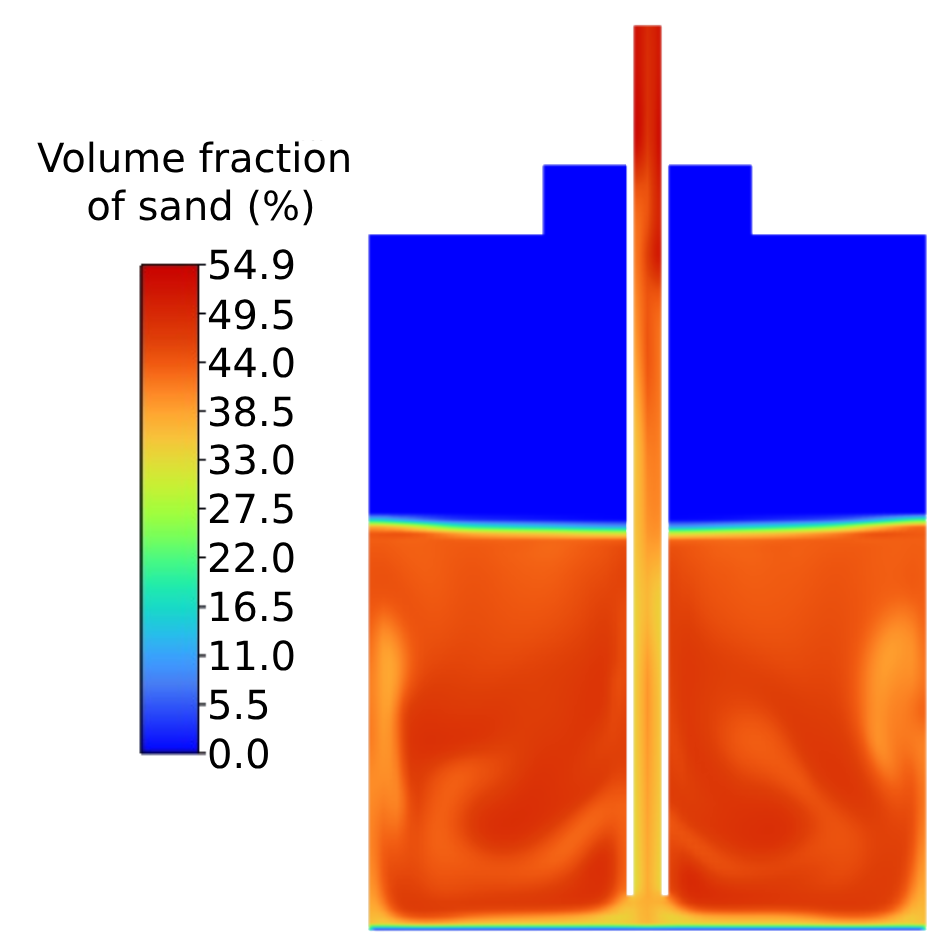
\includegraphics[width=\textwidth]{../report_assets/grav_better.png}
        \caption*{(a) Under Earth's Gravity}
    \end{minipage}
    \hfill
    \begin{minipage}{0.4\textwidth}
        \centering
        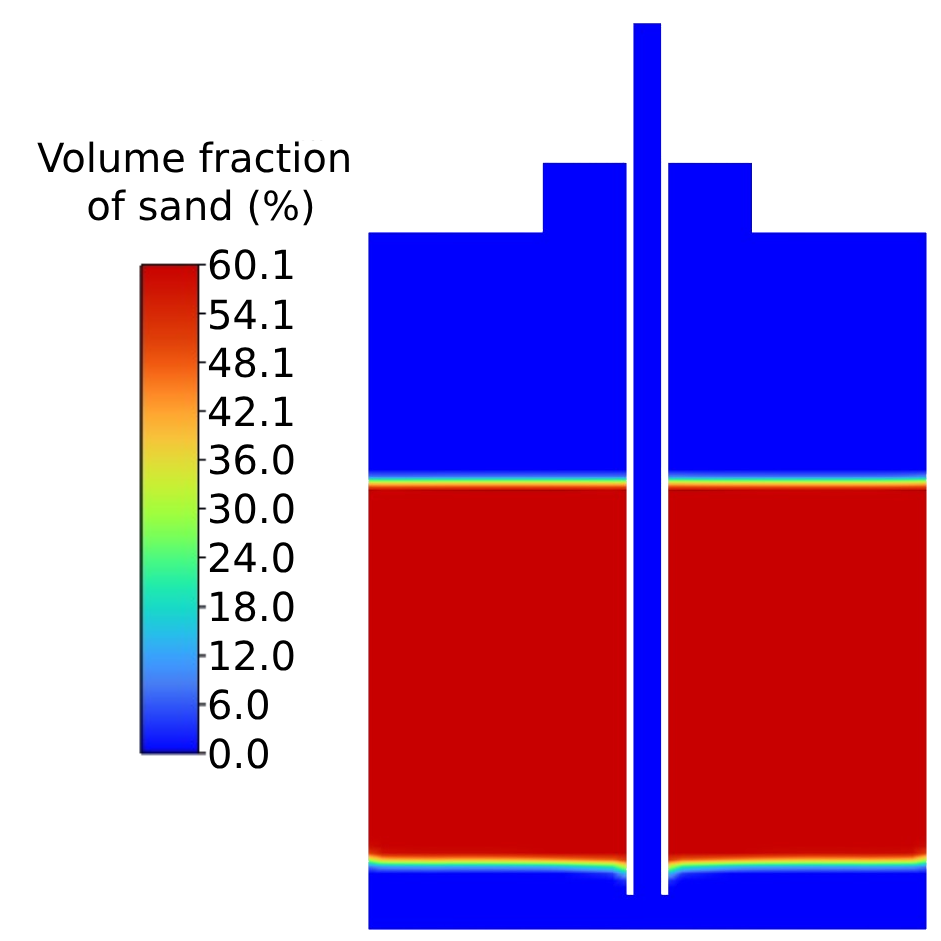
\includegraphics[width=\textwidth]{../report_assets/no_grav_better.png}
        \caption*{(b) Under Microgravity}
    \end{minipage}
    \caption{Phase Density of Old Design after 2 Seconds}\label{fig:old-design-phase-density}
\end{figure}
As shown, there is a marked difference in the location of powder between the two cases. While the powder in the tank under gravity appears to be fully fluidising, the tank in mircogravity is relatively unaffected by the flow. It is thought this is because the steady state flow does not interact with the region of the tank where the powder sits. For rigor, the unprocessed images are provided in \autoref{sec:unprocessed-images}.

\begin{figure}[htbp]
    \centering
    
    \begin{minipage}{0.54\textwidth}
        \centering
        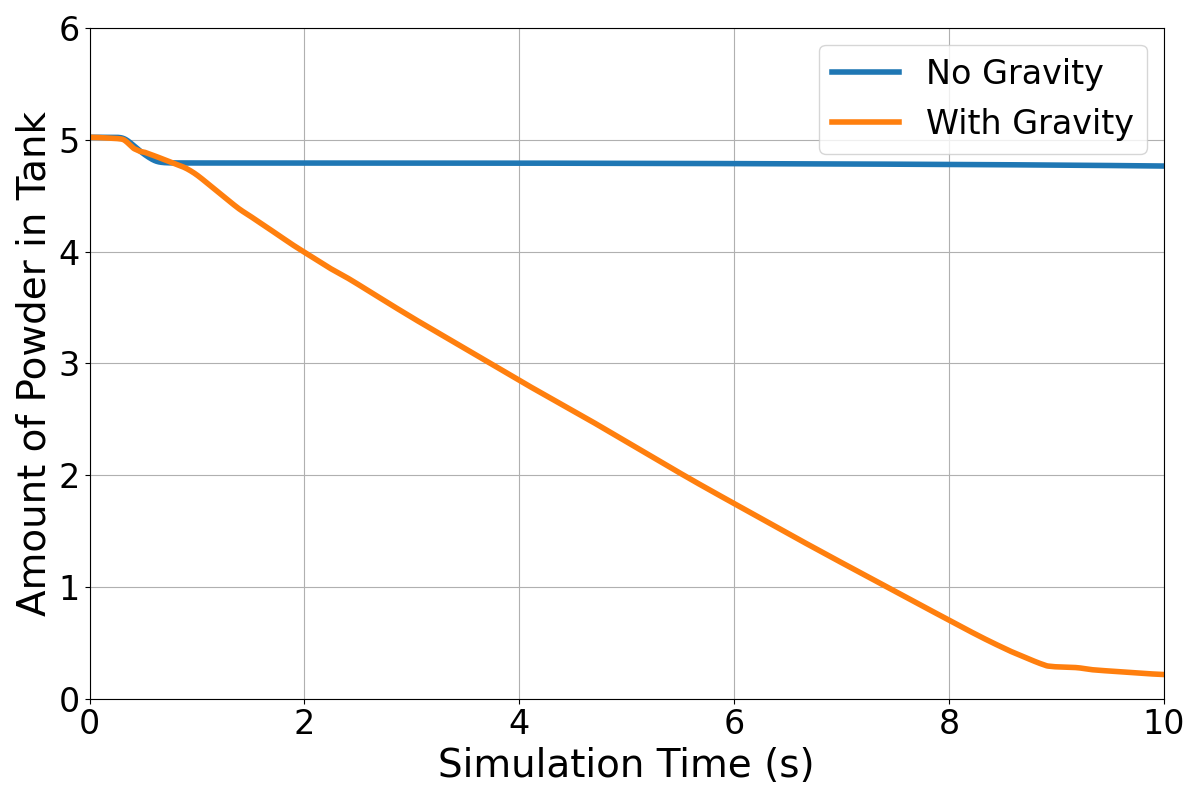
\includegraphics[width=\textwidth]{../report_assets/old_design_out.png}
        \caption{Change of Mass in the Tank Over Time}\label{fig:old-design-mass-change}
    \end{minipage}
    \hfill
    \begin{minipage}{0.4\textwidth}
        \centering
        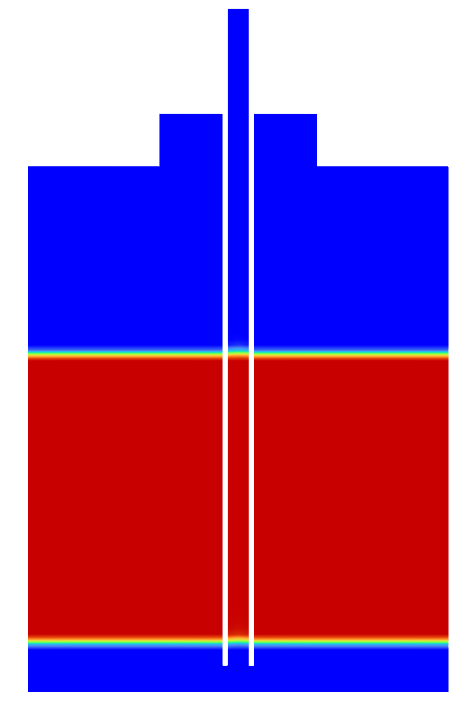
\includegraphics[width=0.6\textwidth]{../report_assets/old_initial.png}
        \caption{Initial Powder Configuration}\label{fig:old-initial}
    \end{minipage}
\end{figure}
\autoref{fig:old-design-mass-change} presents the amount of powder in the tank over time, measured by integrating the volume fraction of the solid phase over the entire geometry. At roughly 0.5s, both simulations show a relatively large drop in powder. This is because of how the simulation was initialised, shown in \autoref{fig:old-initial}, leading to the powder starting in the pipe quickly being expelled from the system. After this, there is a large gap between the two powder dispensing rates, again supporting the hypothesis that the previous design would be less appropriate for microgravity applications and supporting the decision to redesign the tank. 

As mentioned in \autoref{sec:old-design-method}, this analysis was conducted with a relatively coarse mesh which may alter the results. The biggest impact would be not resolving key gradients or incorrect momentum exchange between the two phases. As this geometry is relatively simplistic and the velocity into the system small, it is assumed that there would be minimal impact from not resolving velocity or pressure gradients well enough. However, it is less clear how accurately the momentum exchange is affected by this and was assumed to be valid just based off the authors understanding of the expected behaviour of the system. Given more time this would be an area of focus, conducting a mesh convergence study and running the finer meshes for a longer time should be done to validate this preliminary result. Another area for improvement is using an inlet condition more accurate to the physics. A pressure inlet would have been ideal as this is closer to the physics of the system but due to limitations of the simulation software, there was no way to prevent the powder exiting this inlet. This could be fixed with a user defined function, found through simulating the system with a pressure inlet and no powder, and then transferred to this analysis.

\section{Analysis and Testing Tank Design}\label{sec:pressure-testing}
As mentioned in \autoref{sec:tank-fea-setup}, validation of the tank design was done in two stages, finite element analysis and hand calculations before manufacturing and hydrostatic pressure testing of the full tank once it was made.

The FEA was first ran with 6 bolt holes instead of 8 but was increased as the predicted stress of 6 bolts was above the yield stress of acrylic. As seen in \autoref{fig:fea-results}, the 8 bolt hole configuration shows stresses close to the yeild strength but still below it.
\begin{figure}[htbp]
    \centering

    \begin{minipage}{0.45\textwidth}
        \centering
        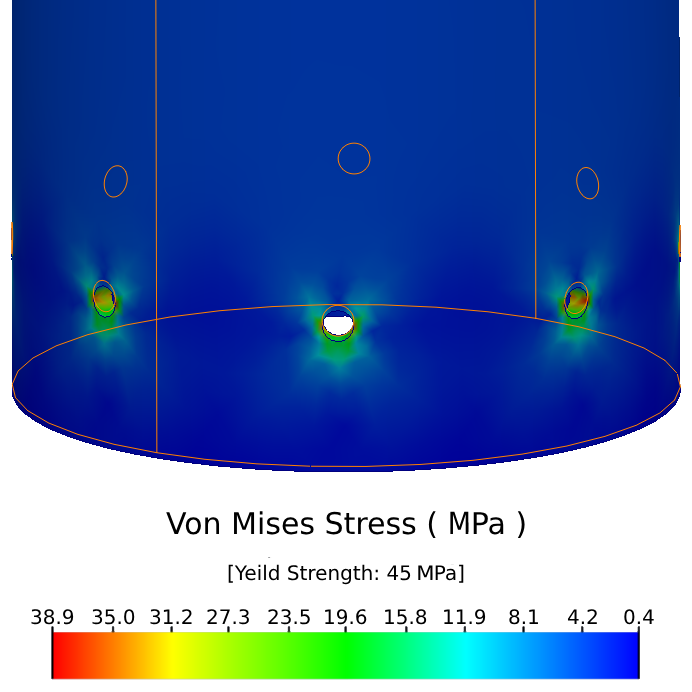
\includegraphics[width=\textwidth]{../report_assets/fine_mesh_results.png}
        \caption*{(a) Fine Mesh}
    \end{minipage}    
    \hfill
    \begin{minipage}{0.45\textwidth}
        \centering
        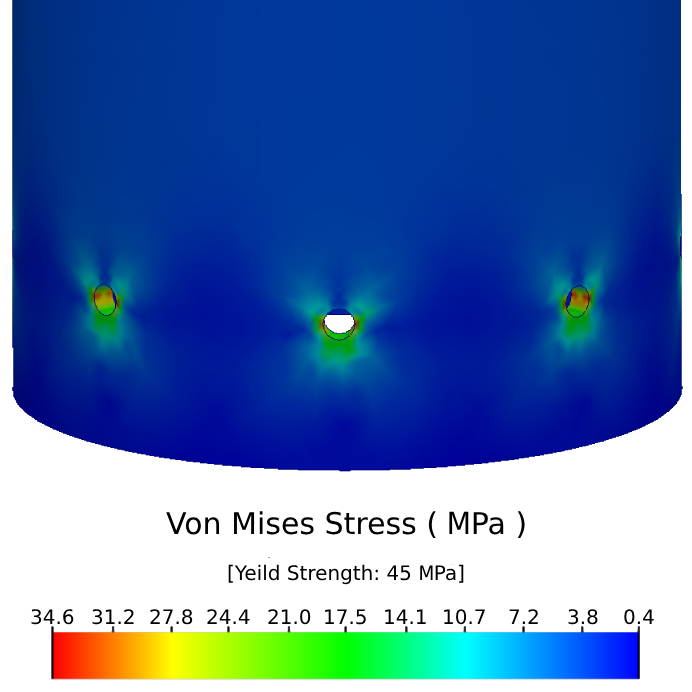
\includegraphics[width=\textwidth]{../report_assets/coarse_mesh_results.png}
        \caption*{(b) More Coarse Mesh}
    \end{minipage}    
    \caption{Results of Tank FEA}\label{fig:fea-results}

\end{figure}  
\autoref{fig:fea-results} (a) shows the original vertices of the tank under no load overlayed in orange over the deformed tank. As there is very little difference between the two, non-linear behaviours from deformation could be ignored. A cylinder is one of the most resiliant shapes to buckling, especially when pressurised so this was not investigated in detail. While there is a slight increase in von mises stress in the more fine mesh, this was assumed to be because of the increased resolution of the boundary between the surface that did have a load applied and the rest of the bolt hole that did not. As the real load is not applied in this way it was determined satisfactory for manufacturing.

The next failure mode checked was hoop stress rupturing, through the use of Lamé's equations. This gave a value of 8.88 GPa of stress at the inner wall and 8.18 GPa of stress at the outer wall. Since it was significantly lower than the bolt hole stress concentration stress, this failure mode was not expected to occur before the others.

After manufacturing, the tank was then hydrostatically pressure tested. The first attempt at pressurising the tank with water resulted in the epoxy-delrin interface seperating. While this was a concern from the design stage, it was expected that reattaching the end cap with a more plastic friendly epoxy and extensive preperation of the bonding delrin surface would solve the issue. This was shown to be true in the subsequent pressure test, seen in \autoref{fig:hydro-results}.
\begin{figure}[htbp]
    \centering

    \begin{minipage}{0.45\textwidth}
        \centering
        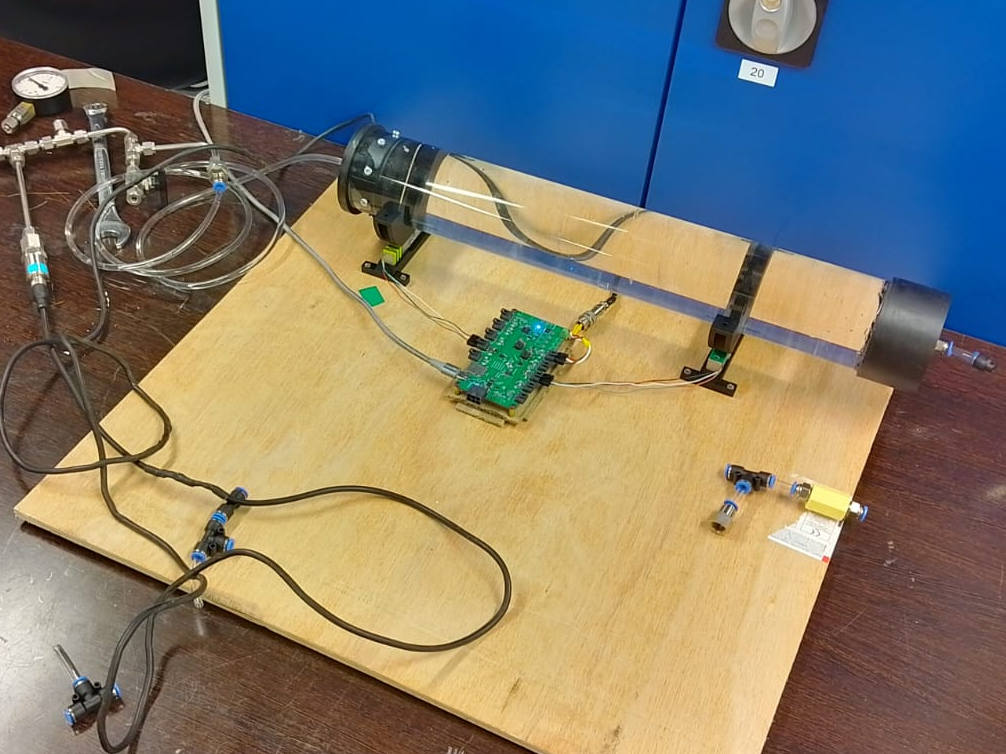
\includegraphics[width=\textwidth]{../report_assets/hydro_testing_setup.png}
        \caption*{(a) Hydrostatic Pressure Testing Setup}
    \end{minipage}    
    \hfill
    \begin{minipage}{0.45\textwidth}
        \centering
        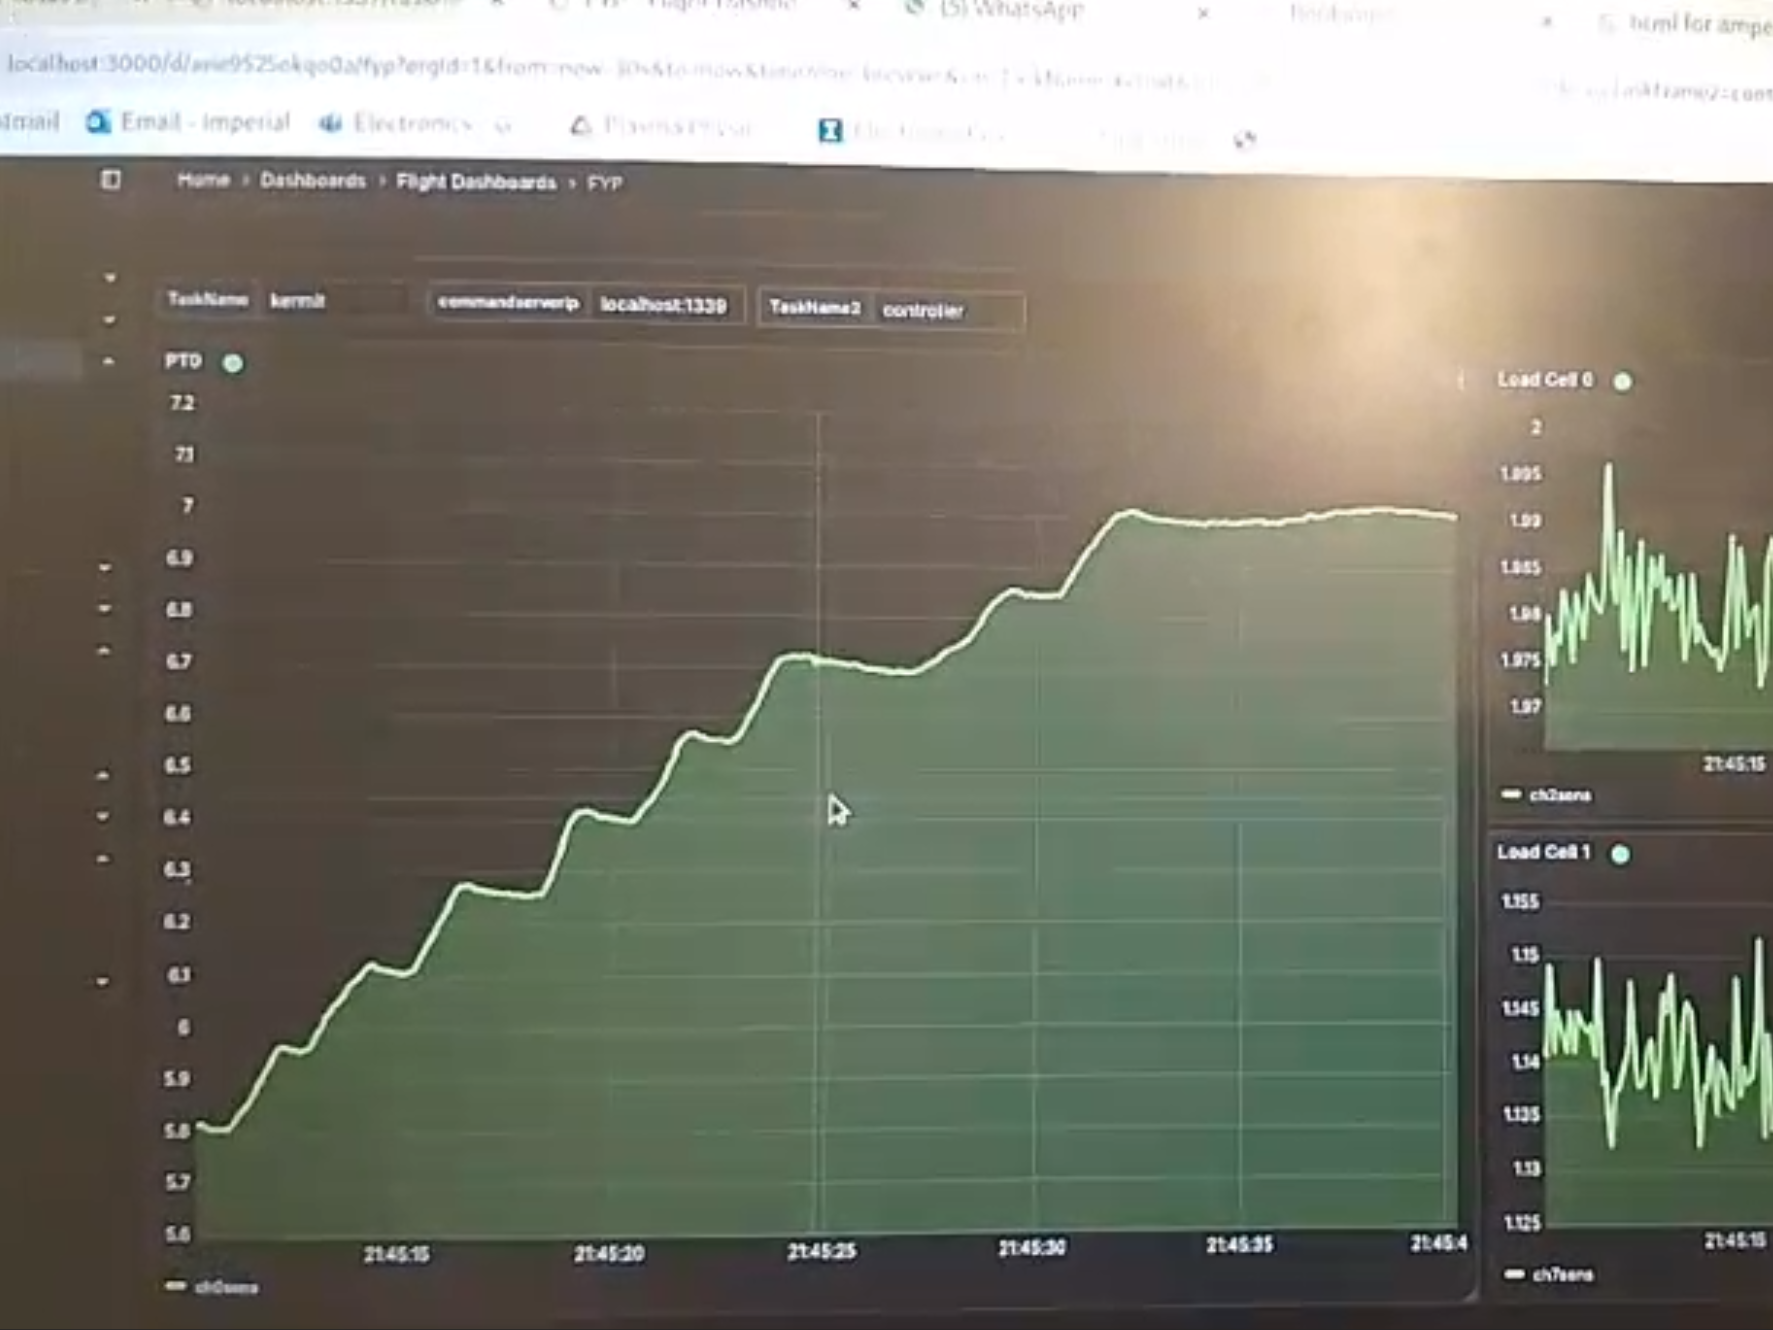
\includegraphics[width=\textwidth]{../report_assets/hydro_grafana.png}
        \caption*{(b) Screenshot of Results from Video}
    \end{minipage}    
    \caption{Results of Tank FEA}\label{fig:hydro-results}

\end{figure}  
Unfortunately, only a video recording of the test was taken and the data being logged was not recorded. A screenshot from this video can be seen in \autoref{fig:hydro-results} (b) and the jagged rise in gauge pressure comes from the actuation of the manual pump. The tank held this 7 bar of gauge pressure for 2 to 3 minutes before the pressure was released. While longer durations under pressure would have given more certainty to the safety of the tank, the strict requirements to vertify the pressure vessel were not needed for the experimentation so were not investigated.

\section{First Test}\label{sec:first-test}
As mentioned in \autoref{sec:piston}, the very first test with was conducted without sand and failed to push the piston down the tank. This quick test was the motivation to characterise the pressure source as it was noted that the pressure readings before and after the tank were lower than expected and changed slower than expected. This meant that the failure mode of the piston crumpling was discounted and the future piston designs ignored this possibility. After characterisation of the pressure source, the second piston was tested, seen in \autoref{fig:first-test}. 

\begin{figure}[htbp]
    \centering
    
    \begin{minipage}{0.6\textwidth}
        \centering
        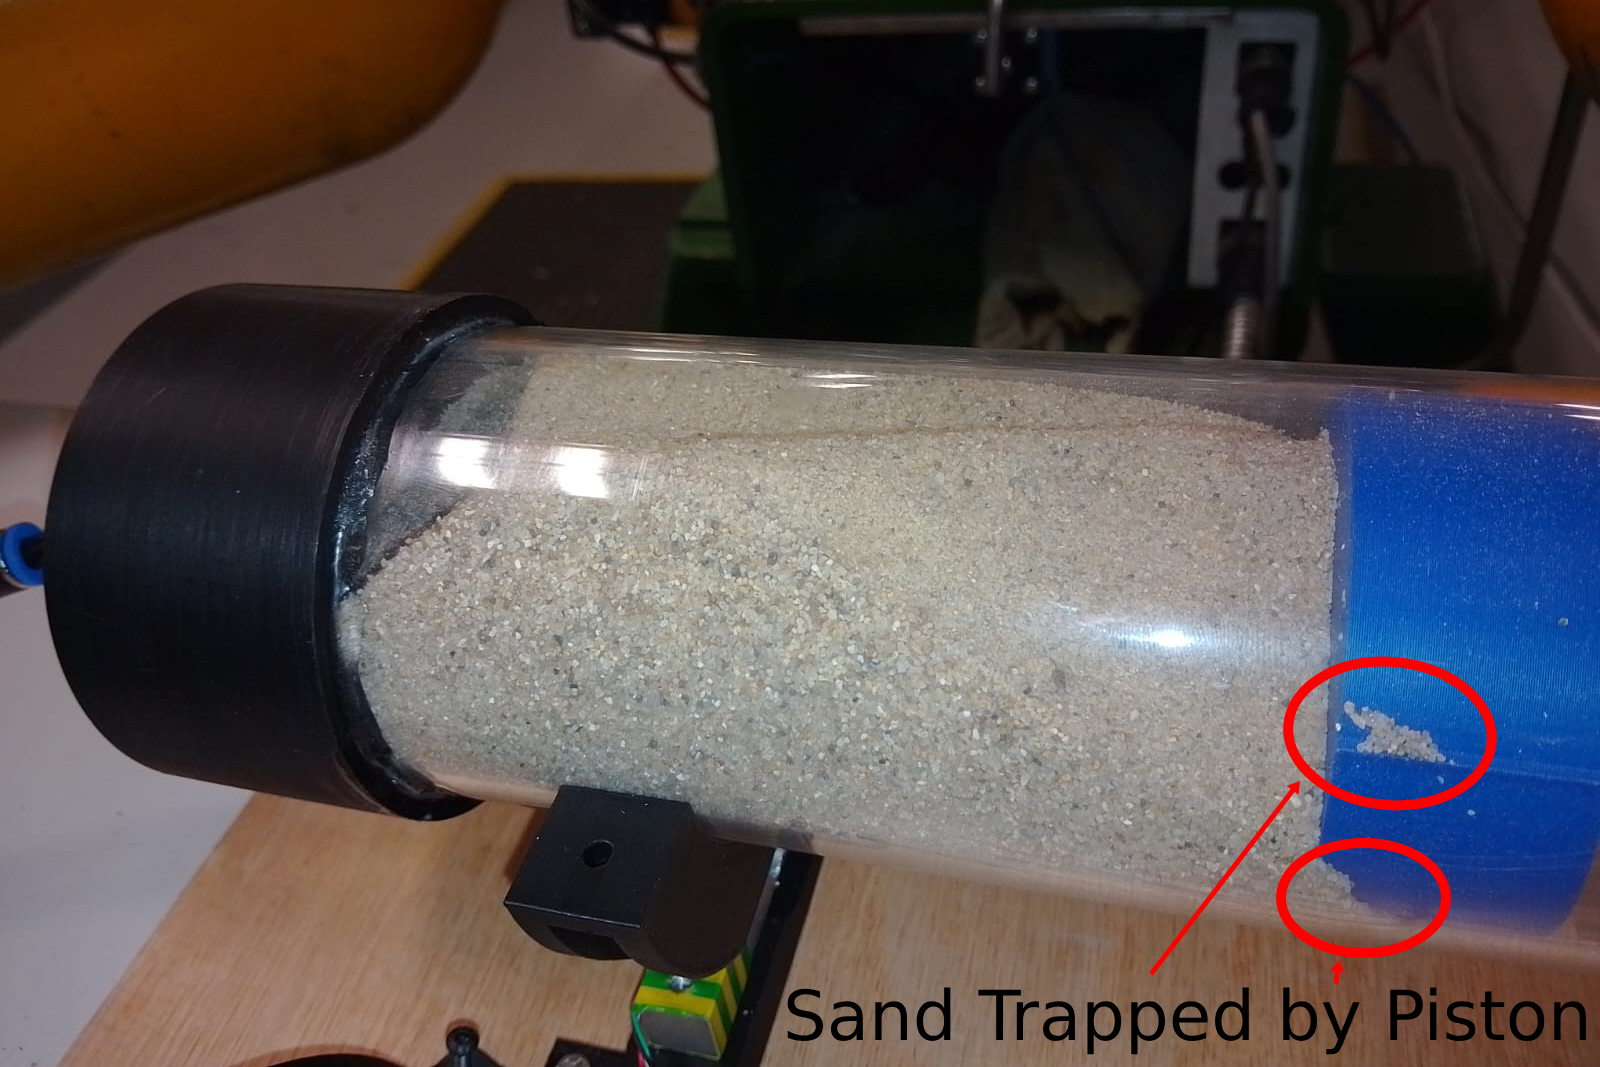
\includegraphics[width=\textwidth]{../report_assets/first_test.png}
        \caption{Result of First Powder Test}\label{fig:first-test}
    \end{minipage}
    
\end{figure}
The piston started far down the tank and was successfully pushed towards the outlet. At the point it reached the sand, it became stuck, as the unpacked grains formed a wedge under the piston and caused it to jam into the side walls of the tank. With the powder not compacted against the outlet, ratholing began to occur as the gas entrained the sand particles through the outlet, highlighting an alternate dispensing regime to be avoided. The gap between the piston and the walls was designed to be 1mm so it is expected that this specific issue would not have occured with a finer grain sand. While purchasing finer grain sand or crushing down the current sample were considered, it was decided that a new design would be investigated as this was not something seen in the literature and would be much easier to characterise the friction. A full analysis of the piston was of great interest but given the limited time of the project, was deemed out of the scope. 

\section{Characterising Pressure Source}\label{sec:static_test}
\subsection{Initial Test}
The first step in characterising the system was to investigate the static pressure losses present in the tank without a piston or any powder. This immediately presented a problem as the static pressure readings, given a gas source with a stagnation pressure of 4 to 6 bar, were far below expected, as seen in figure \autoref{fig:static-pressure-drop}. 
\begin{figure}[htbp]
    \centering

    \begin{minipage}{0.45\textwidth}
        \centering
        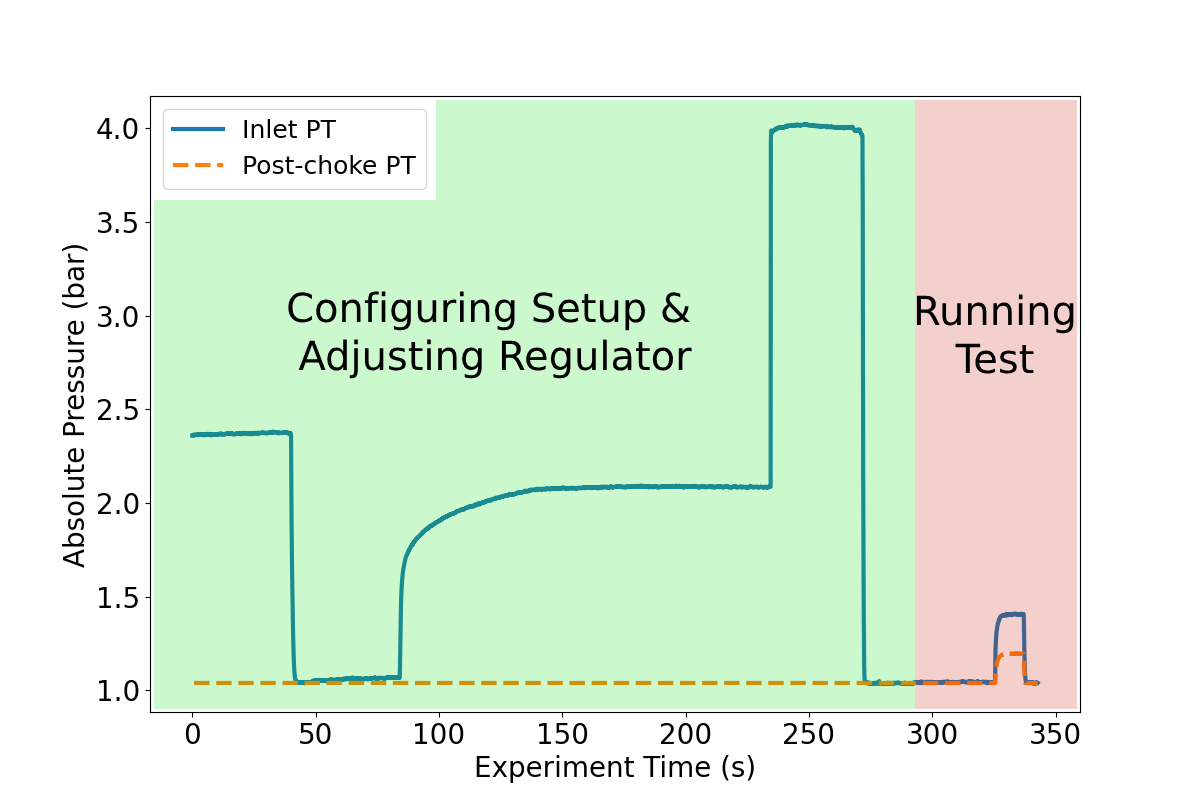
\includegraphics[width=\textwidth]{../report_assets/3_bar_static_full.png}
        \caption*{(a) Full 4 bar Test}
    \end{minipage}    
    \hfill
    \begin{minipage}{0.45\textwidth}
        \centering
        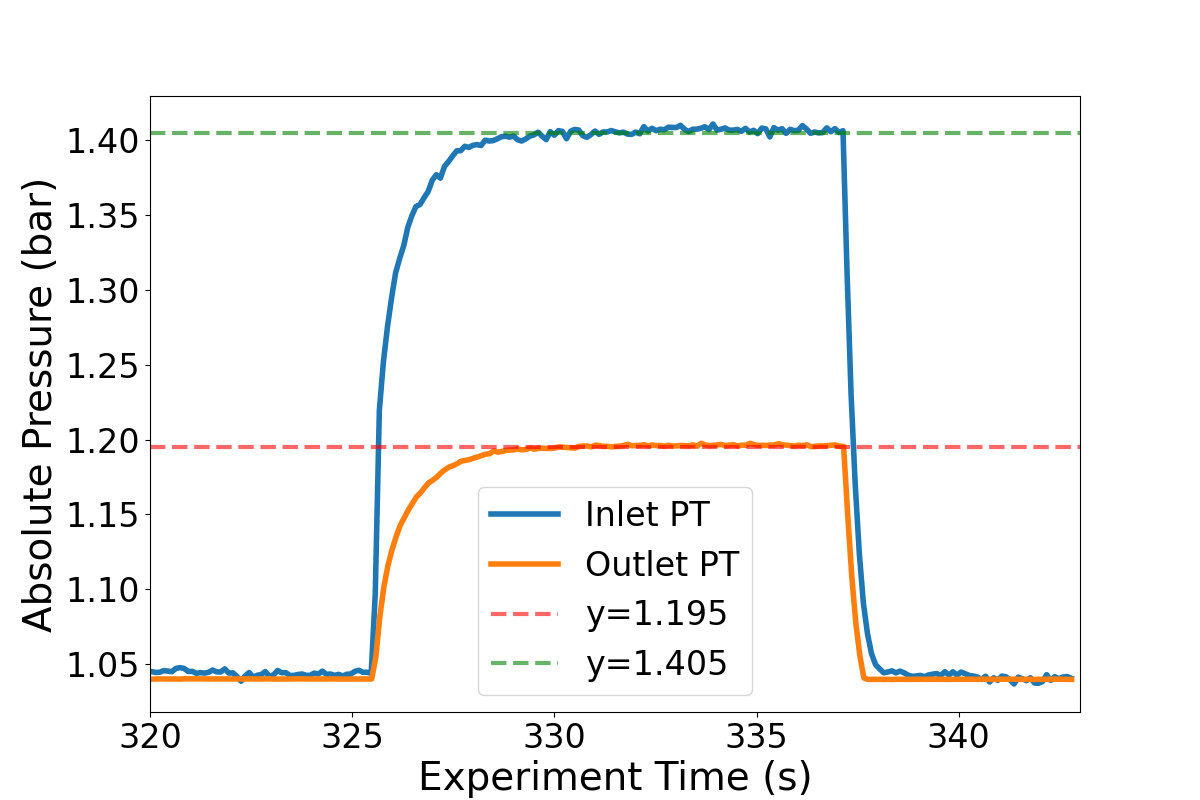
\includegraphics[width=\textwidth]{../report_assets/3_bar_static.png}
        \caption*{(b) Static Pressure from 4 bar}
    \end{minipage}    
    \begin{minipage}{0.45\textwidth}
        \centering
        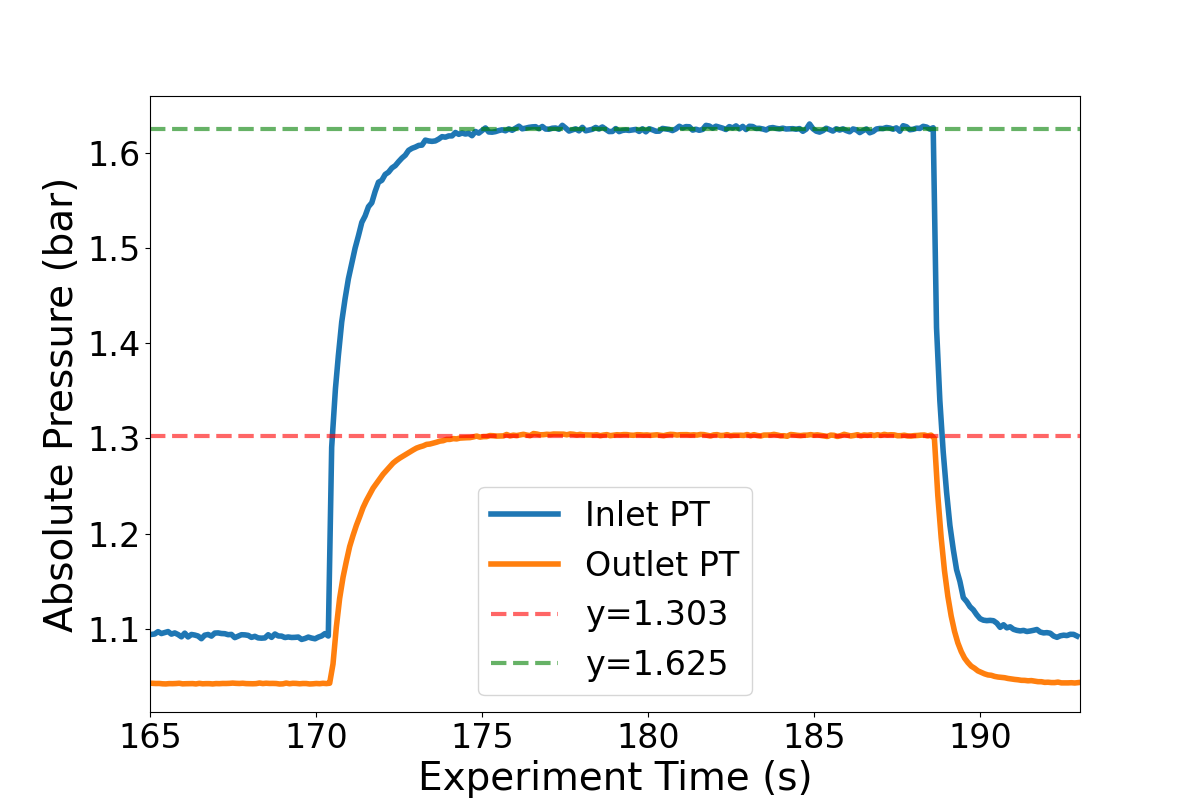
\includegraphics[width=\textwidth]{../report_assets/4_bar_static.png}
        \caption*{(c) Static Pressure from 5 bar}
    \end{minipage}    
    \hfill
    \begin{minipage}{0.45\textwidth}
        \centering
        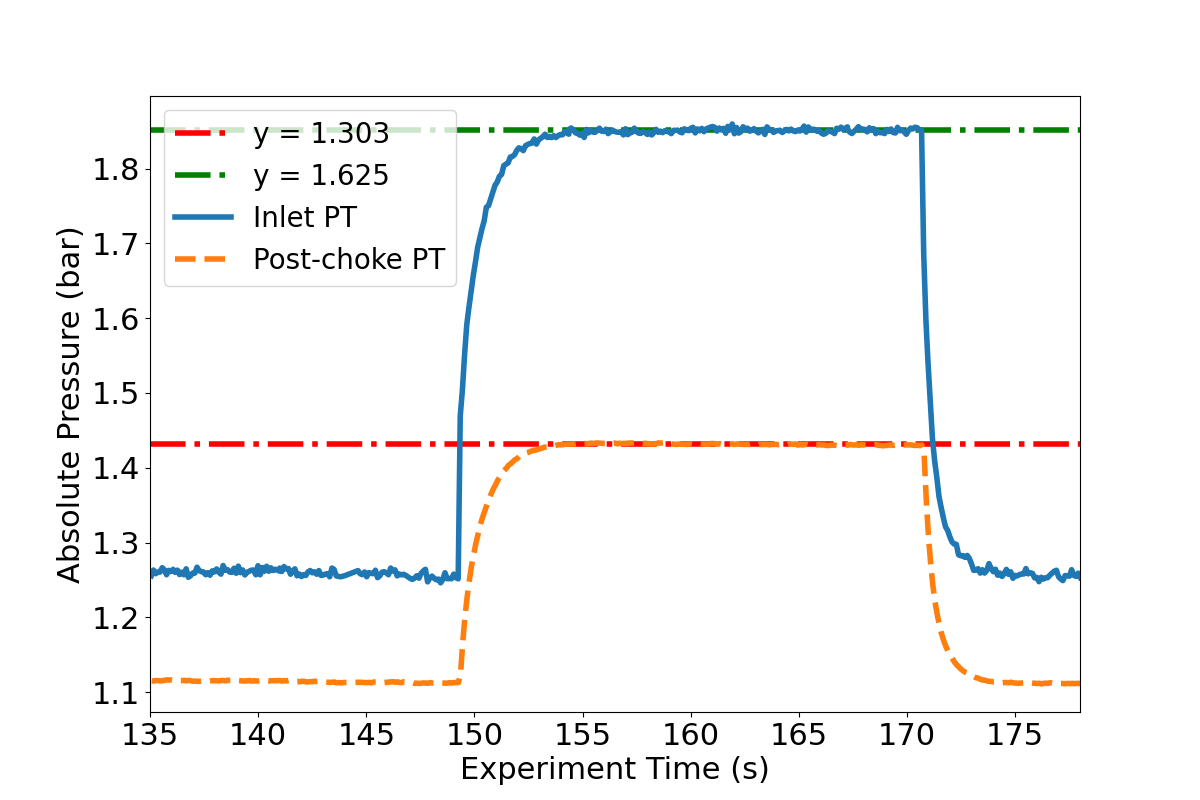
\includegraphics[width=\textwidth]{../report_assets/5_bar_static.png}
        \caption*{(d) Static Pressure from 6 bar}
    \end{minipage}    

    \caption{Static Pressure Readings Before and After the Tank at Different Pressures}\label{fig:static-pressure-drop}
\end{figure}    
If the compressed air line was truely supplying a stagnation pressure of 4 bar, through isentropic flow relations the data implies that the mach number of the flow is 1.3 which is unlikely.

As seen in \autoref{fig:static-pressure-drop} (a), the regulator was able to control the static pressure to 4 bar when the system was closed. When the system opens, one could expect that the regulator would maintain this 4 bar static pressure and only static pressure losses in the system and acceleration of the flow beyond the regulator would reduce it somewhat. However, by the time the flow reached the pressure transducer before the tank, the static pressure had dropped to 1.4 bar. 

Assuming the flow was mach 1 through the nylon pipe, this would imply a stagnation pressure of roughly 2 bar not the 4 bar initially desired. As seen in~\autoref{fig:static-pressure-drop} (c) and (d), this behaviour was persistant at higher inlet pressures, dont really know why rn but justify when i do

\subsection{Further Investigation}
In an attempt to diagnose this behaviour, follow up tests were conducted. As seen in figure the performance was much worse giving even lower static pressure readings. 
\begin{figure}[htbp]
    \centering

    \begin{minipage}{0.45\textwidth}
        \centering
        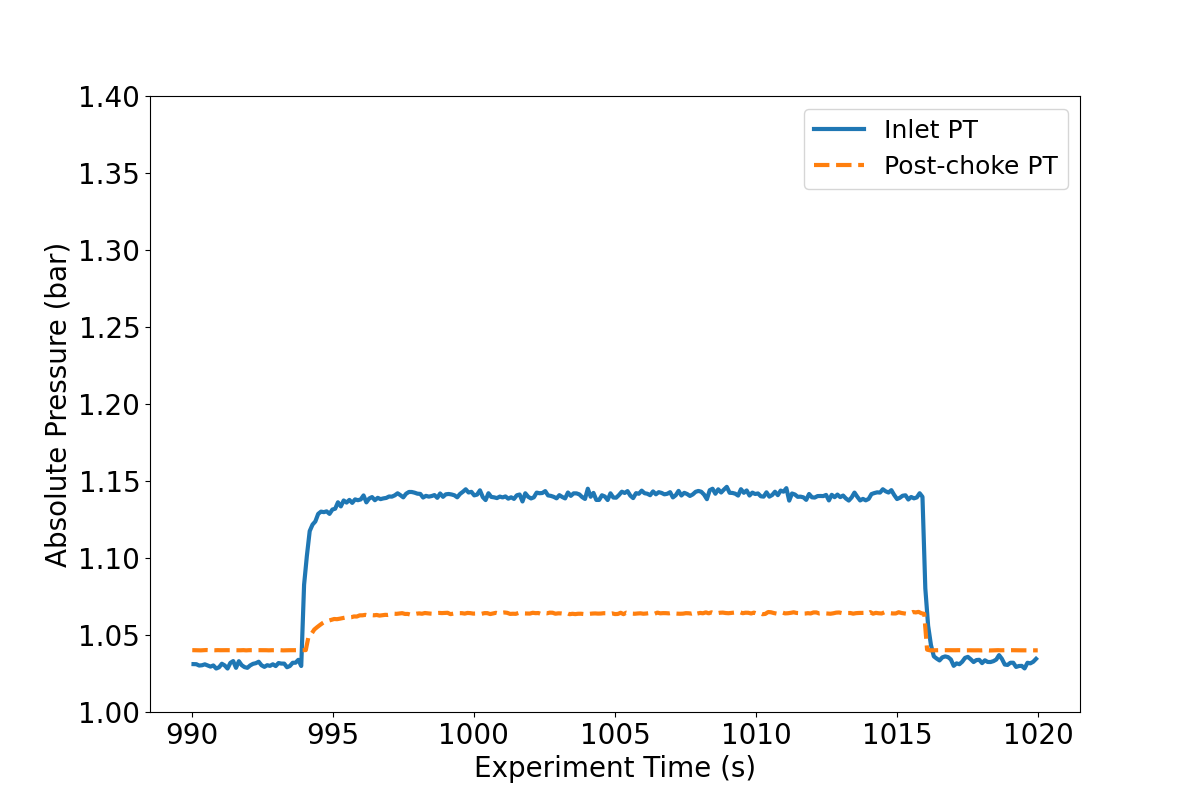
\includegraphics[width=\textwidth]{../report_assets/3_bar_static_new_reg.png}
        \caption{New regulator.}\label{fig:static-pressure-drop-new-reg}
    \end{minipage}    
    \hfill
    \begin{minipage}{0.45\textwidth}
        \centering
        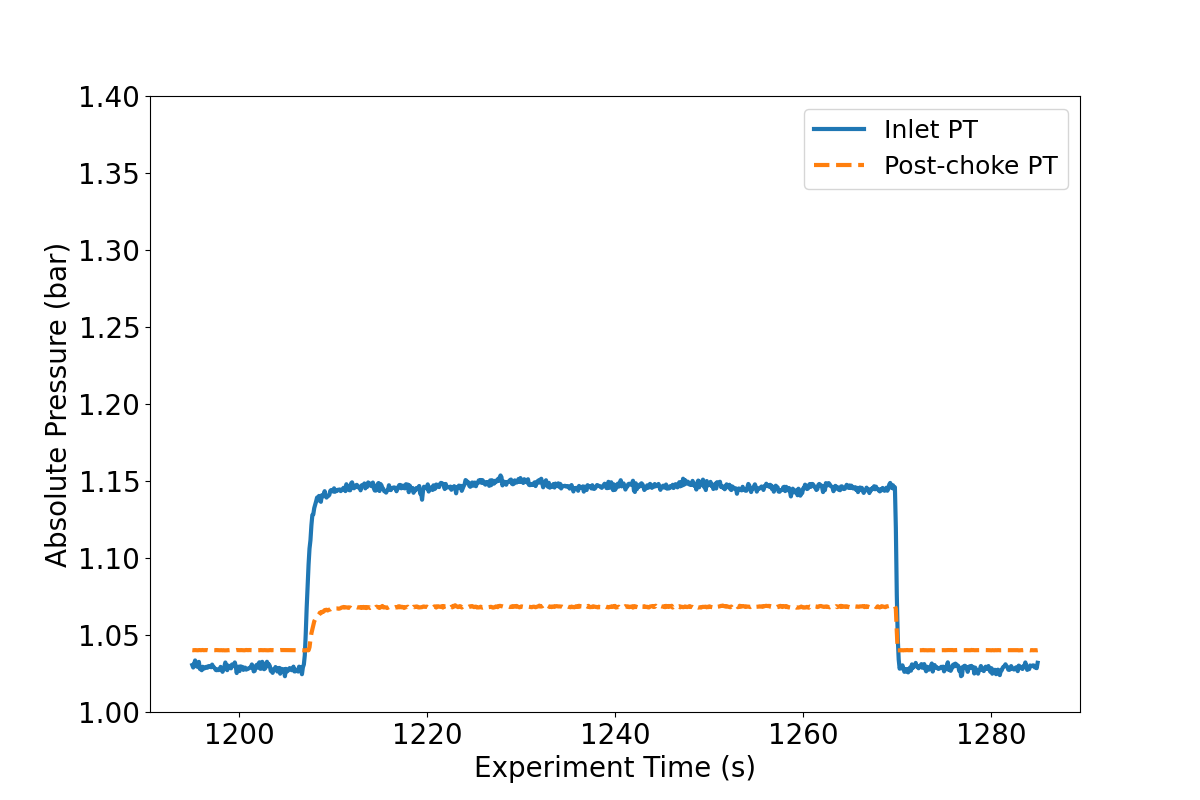
\includegraphics[width=\textwidth]{../report_assets/3_bar_static_no_solenoid.png}
        \caption{New regulator + no solenoid.}\label{fig:static-pressure-drop-no-solenoid}
    \end{minipage}    

\end{figure}    
As a final attempt, the solenoid valve was removed from the set up to verify that this wasnt choking the flow or somehow drastically decreasing static pressure somehow. Again, seen in fig 6, this performed similarly to the setup containing the regulator so wasn't the cause of the behaviour and the system diagram was reverted to \autoref{fig:systems-diagram}.

\subsection{Simulation}
The 2D axisymmetric analysis of the empty tank seemed to support the idea that the stagnation pressure supplied into the system was less than 4 bar. The pressure gradient, seen in \autoref{fig:static-pressure-drop-fluent}, produces comparable results to the readings from the pressure transducers experimentally. 
\begin{figure}[htbp]
    \centering
    
    \begin{minipage}{0.9\textwidth}
        \centering
        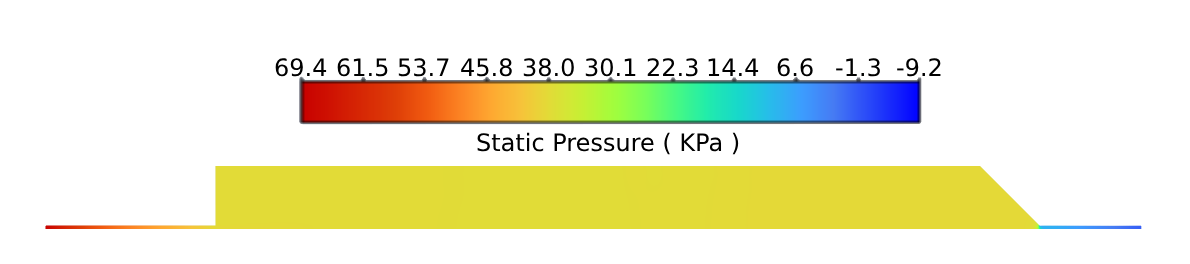
\includegraphics[width=\textwidth]{../report_assets/static_pressure_sim_results.png}
        \caption{Static Pressure of Empty Tank Simulation}\label{fig:static-pressure-drop-fluent}
    \end{minipage}    
    
\end{figure}    
The values recorded at the pressure reading regions were 1.46 bar before the tank and 1.06 bar after the tank. While this is close to the experimental results, the outlet is notably lower suggesting this still does not fully explain the behaviour.

The velocity of the flow was also found in the simulation, seen in \autoref{fig:velocity-magnitude-fluent}.
\begin{figure}[htbp]
    \centering
    
    \begin{minipage}{0.9\textwidth}
        \centering
        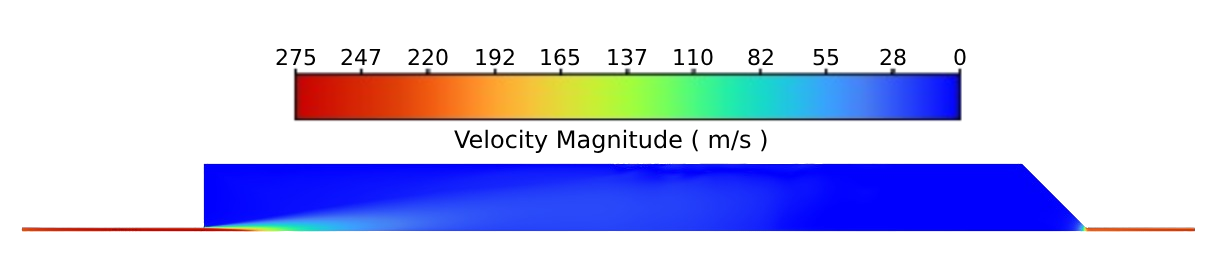
\includegraphics[width=\textwidth]{../report_assets/pressure_characterisation_vel.png}
        \caption{Velocity Magnitude of Empty Tank Simulation}\label{fig:velocity-magnitude-fluent}
    \end{minipage}    
    
\end{figure}    
In the 0.1m of pipe, the flow has already accelerated to 275m/s which supports the idea that the flow within the pipes held a lot of the stagnation pressure as dynamic pressure and this is why the static pressure readings were so low.
\subsection{Stagnation pressure values}
Given the unreliability of the pressure gauge, a number of assumptions were made to determine the stagnation pressure and allow for analysis of mass flow rate against pressure. Assuming that the flow was choked within the tubes, having a velocity of 343m/s, the isentropic relations give that p/p0 =  0.52828178
\begin{table}[htbp]
    \centering
    \begin{tabular}{|c|c|c|}
        \hline
        Pressure Regulator Setting (bar) & Static Pressure at Inlet (bar) &  Stagnation Pressure (bar) \\
        \hline
        4 & 1.405 & 2.66 \\
        5 & 1.625 & 3.08 \\
        6 & 1.852 & 3.51 \\
        \hline
    \end{tabular}    
    \caption{Summary of static and stagnation pressures for different tests.}
    \label{tab:static-stag-pressures}
\end{table}    


\newpage
\section{Mass Flow Rate Experiment}
\subsection{Results from an Inlet Pressure of 4 bar}
\vfill

\begin{figure}[htbp]
    \centering

    \begin{minipage}{0.32\textwidth}
        \centering
        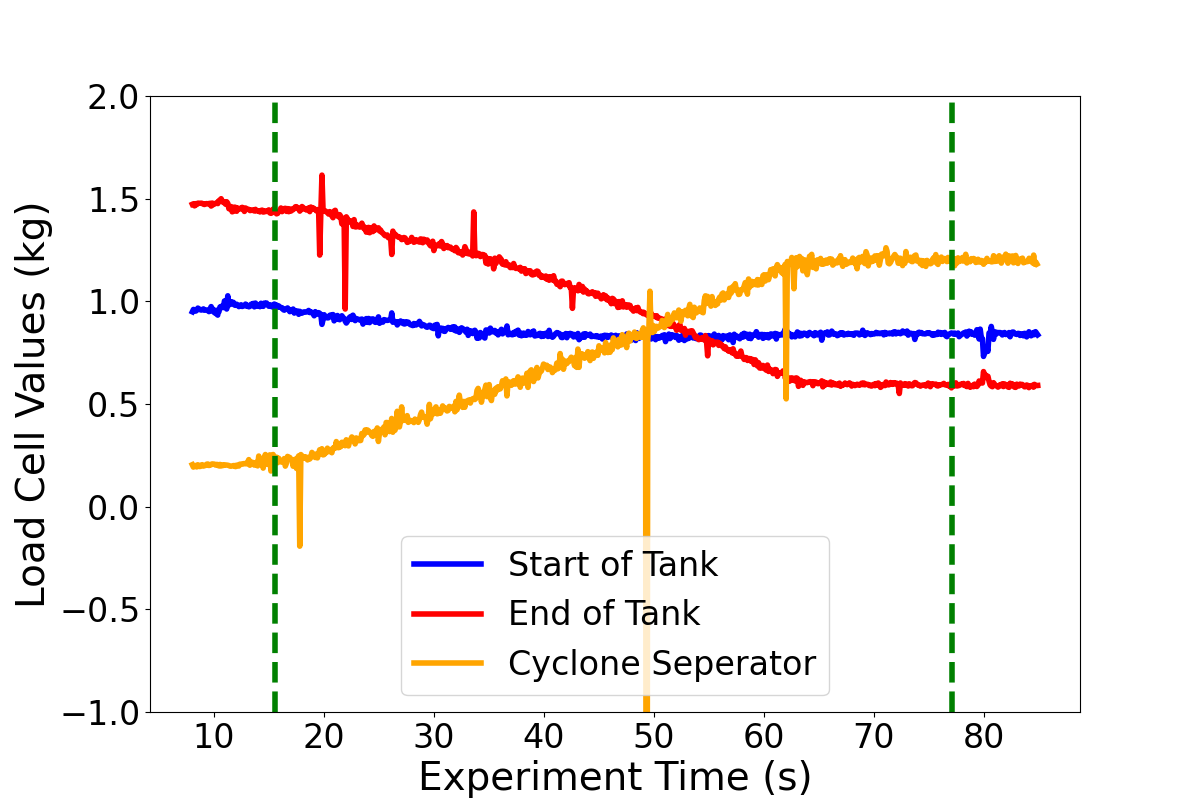
\includegraphics[width=\textwidth]{../report_assets/41_raw_mass.png}
        \caption*{(a) Raw Load Cell Readings}
    \end{minipage}
    \hfill
    \begin{minipage}{0.32\textwidth}
        \centering
        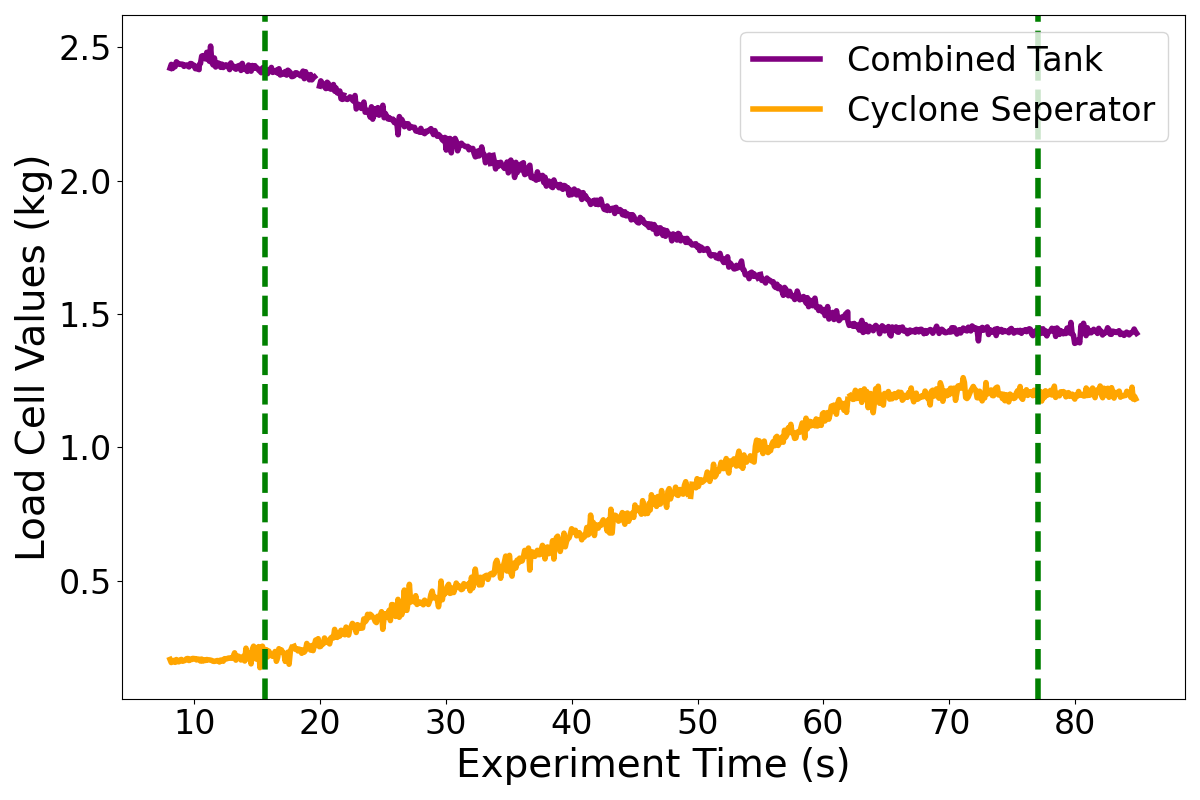
\includegraphics[width=\textwidth]{../report_assets/41_clean_mass.png}
        \caption*{(b) Cleaned Mass Change}
    \end{minipage}
    \hfill
    \begin{minipage}{0.32\textwidth}
        \centering
        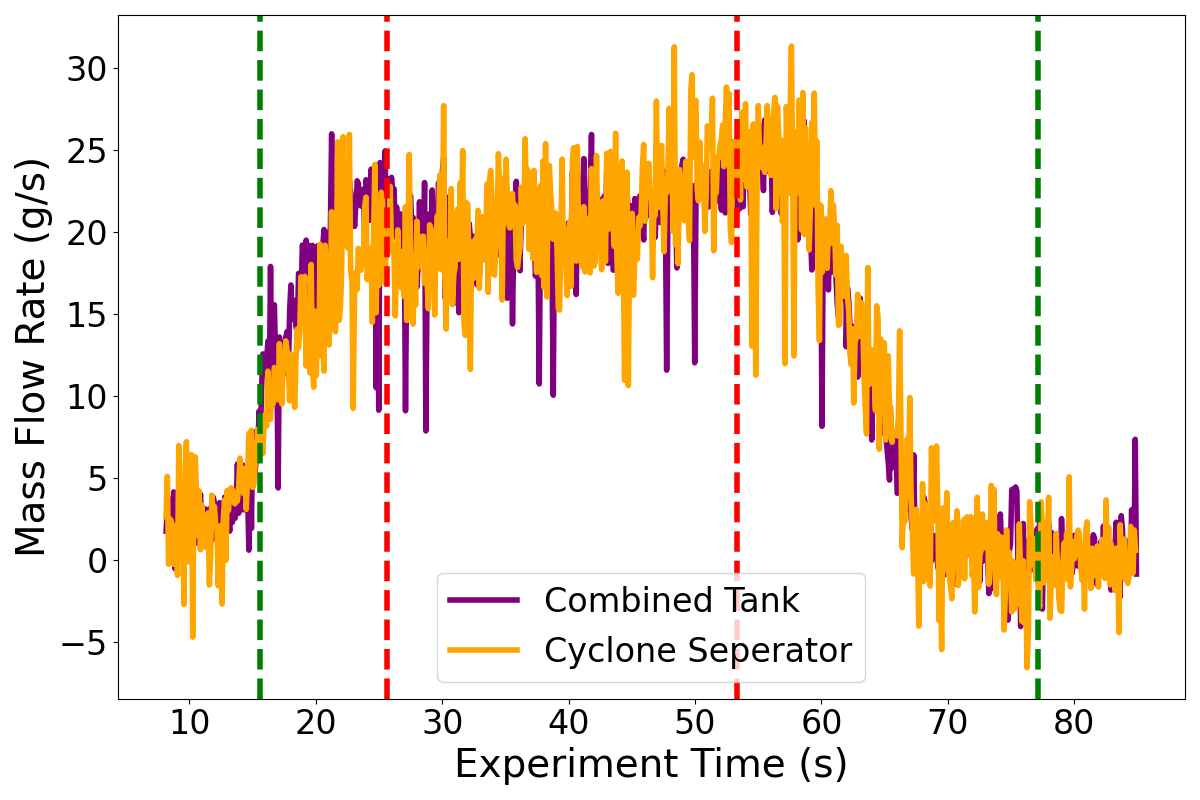
\includegraphics[width=\textwidth]{../report_assets/41_clean_flow_100.png}
        \caption*{(c) Mass Flow Rate}
    \end{minipage}
    \caption{1st Test 4 Bar Inlet}

\end{figure}\label{fig:41}
\vfill
\begin{figure}[htbp]
    \centering

    \begin{minipage}{0.32\textwidth}
        \centering
        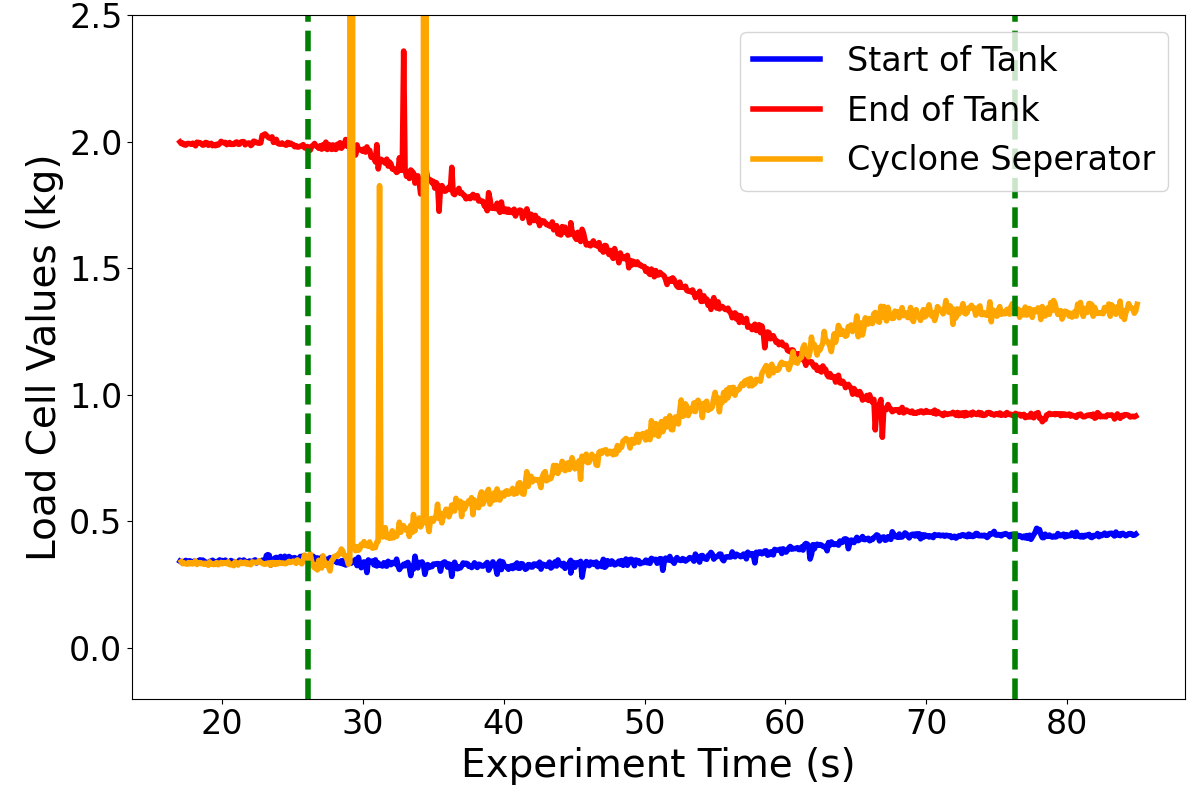
\includegraphics[width=\textwidth]{../report_assets/42_raw_mass.png}
        \caption*{(a) Raw Load Cell Readings}
    \end{minipage}
    \hfill
    \begin{minipage}{0.32\textwidth}
        \centering
        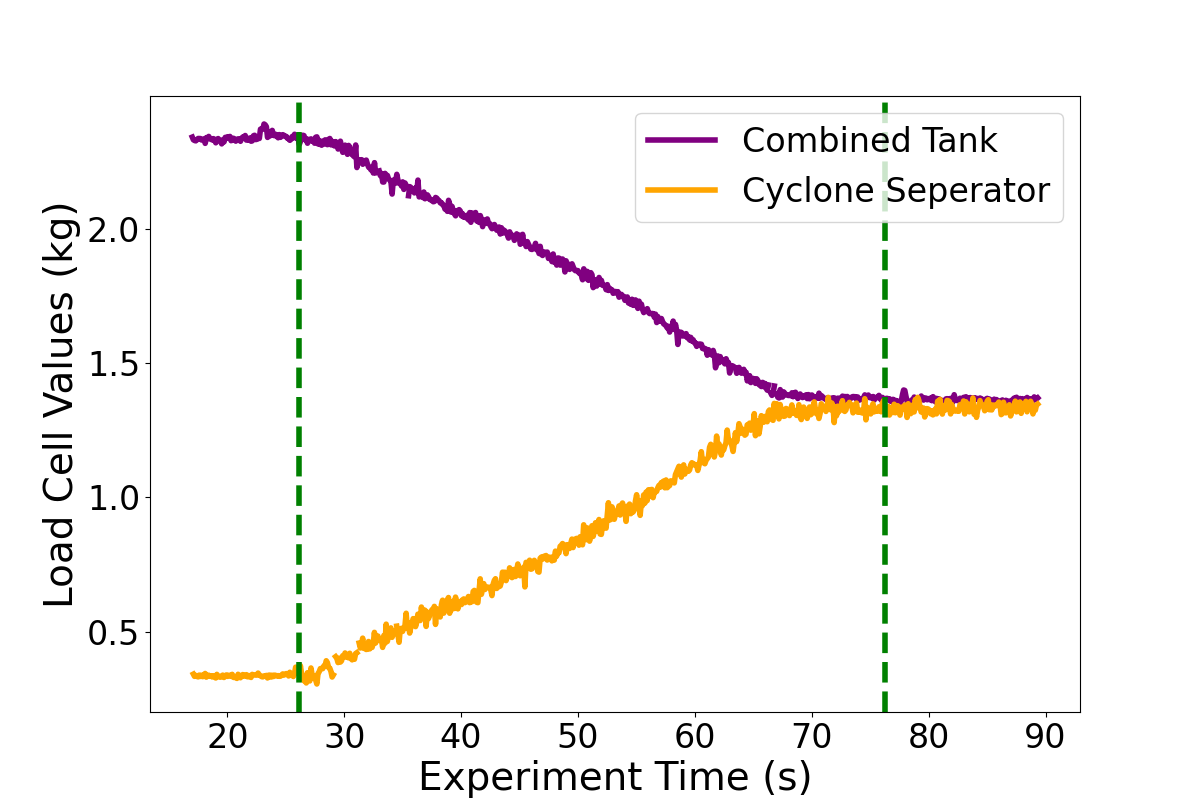
\includegraphics[width=\textwidth]{../report_assets/42_clean_mass.png}
        \caption*{(b) Cleaned Mass Change}
    \end{minipage}
    \hfill
    \begin{minipage}{0.32\textwidth}
        \centering
        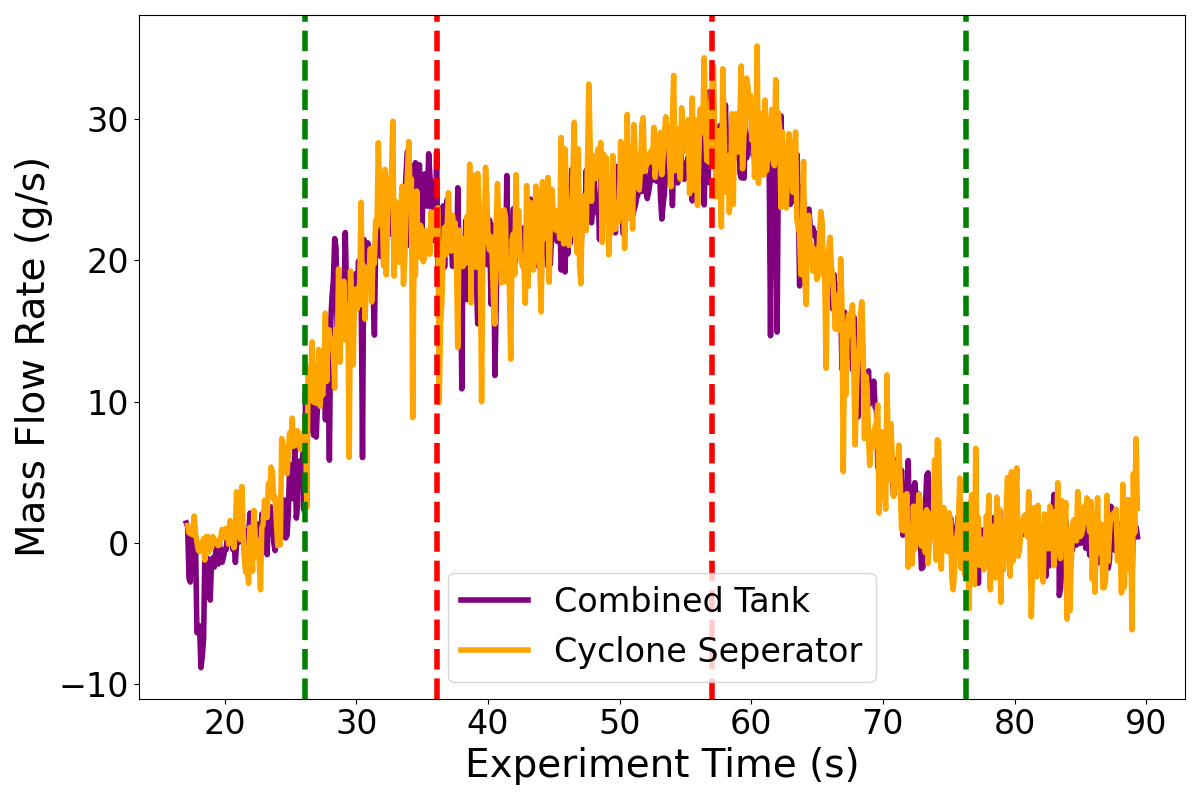
\includegraphics[width=\textwidth]{../report_assets/42_clean_flow_100.png}
        \caption*{(c) Mass Flow Rate}
    \end{minipage}
    \caption{2nd Test 4 Bar Inlet}
    
\end{figure}\label{fig:42}
\vfill
\begin{figure}[htbp]
    \centering

    \begin{minipage}{0.32\textwidth}
        \centering
        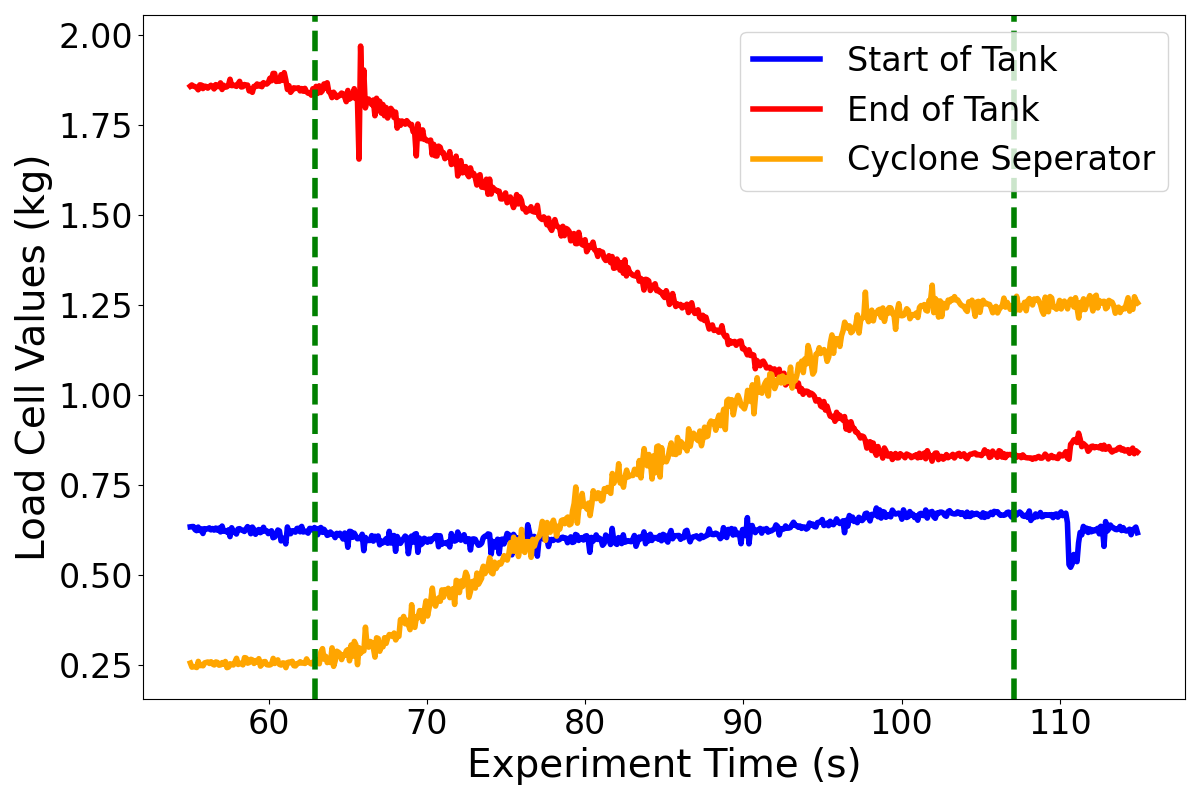
\includegraphics[width=\textwidth]{../report_assets/43_raw_mass.png}
        \caption*{(a) Raw Load Cell Readings}
    \end{minipage}
    \hfill
    \begin{minipage}{0.32\textwidth}
        \centering
        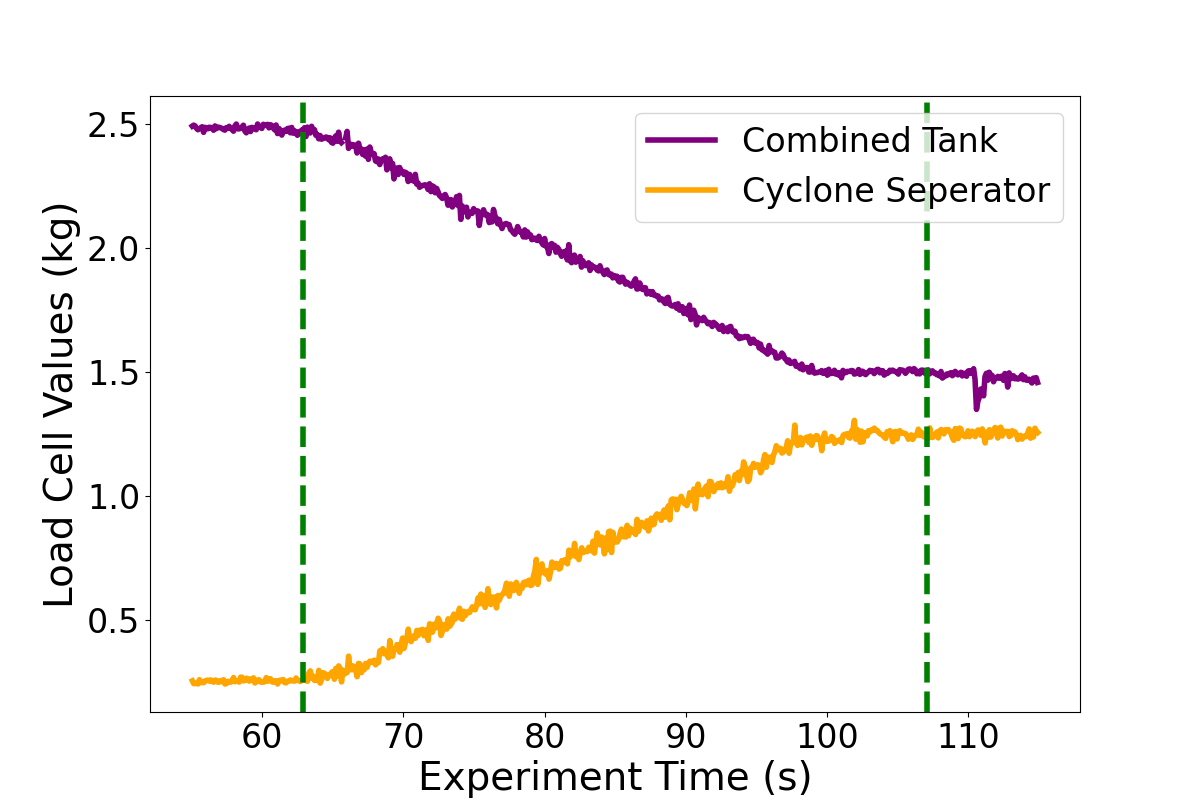
\includegraphics[width=\textwidth]{../report_assets/43_clean_mass.png}
        \caption*{(b) Cleaned Mass Change}
    \end{minipage}
    \hfill
    \begin{minipage}{0.32\textwidth}
        \centering
        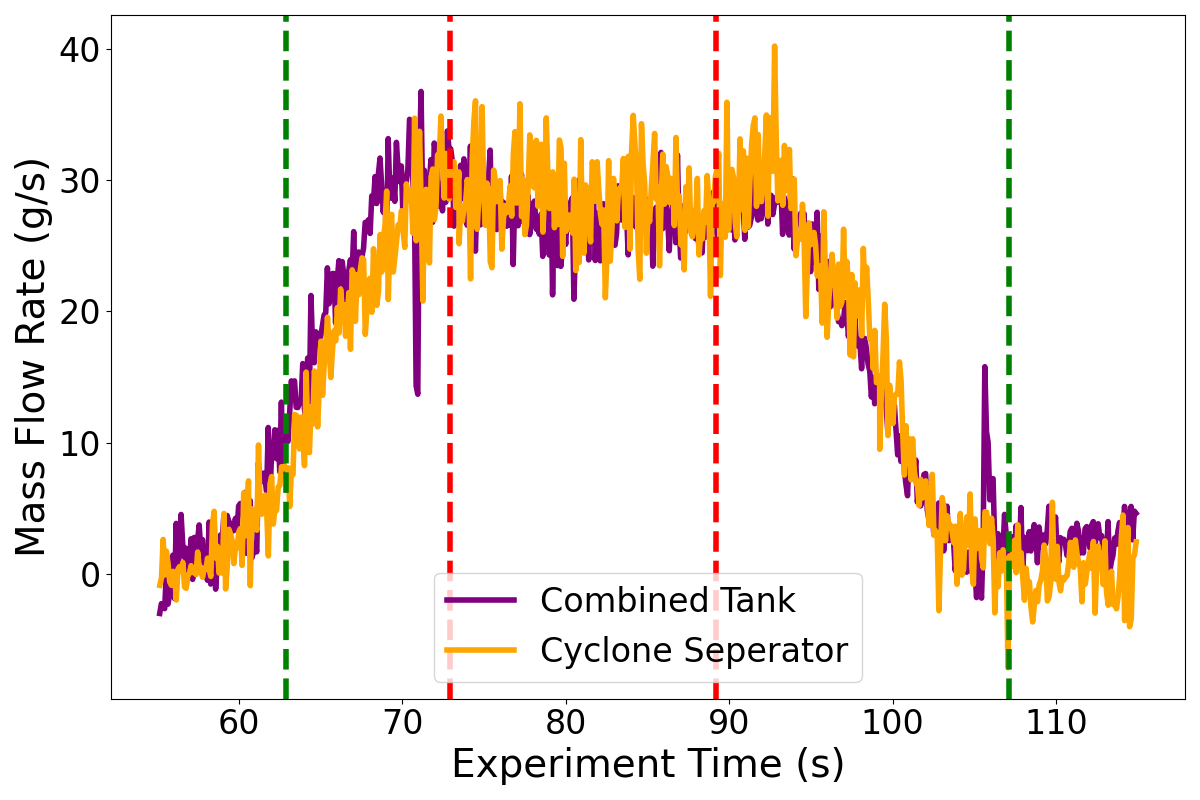
\includegraphics[width=\textwidth]{../report_assets/43_clean_flow_100.png}
        \caption*{(c) Mass Flow Rate}
    \end{minipage}
    \caption{3rd Test 4 Bar Inlet}
    
\end{figure}\label{fig:43}
\vfill

\newpage

\subsection{Results from an Inlet Pressure of 5 bar}
\vfill
\begin{figure}[htbp]
    \centering

    \begin{minipage}{0.32\textwidth}
        \centering
        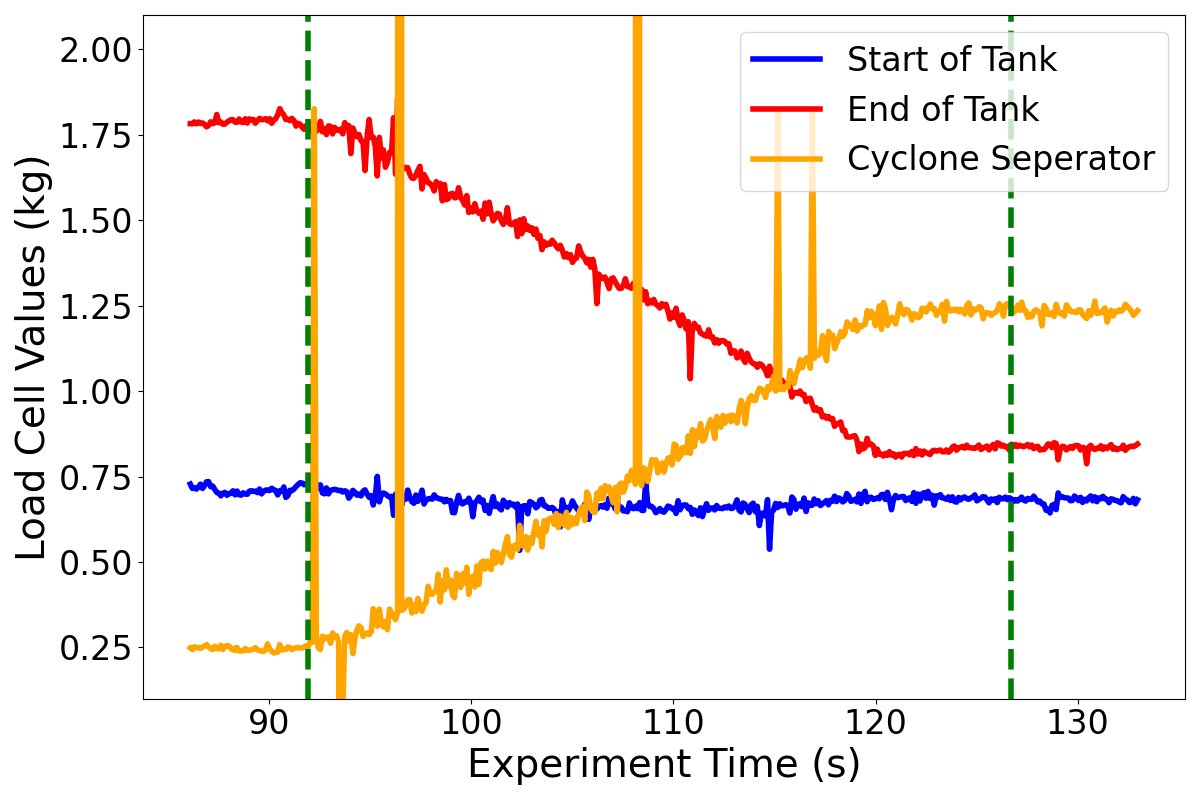
\includegraphics[width=\textwidth]{../report_assets/51_raw_mass.png}
        \caption*{(a) Raw Load Cell Readings}
    \end{minipage}
    \hfill
    \begin{minipage}{0.32\textwidth}
        \centering
        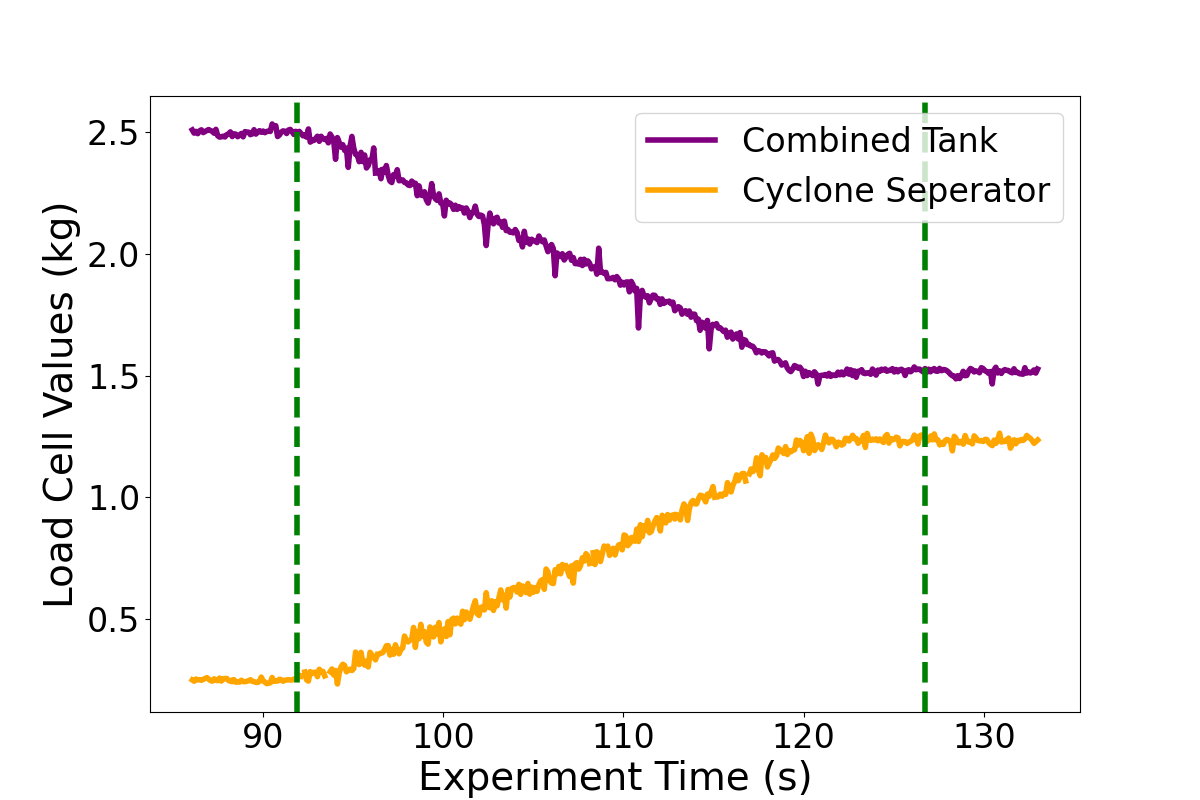
\includegraphics[width=\textwidth]{../report_assets/51_clean_mass.png}
        \caption*{(b) Cleaned Mass Change}
    \end{minipage}
    \hfill
    \begin{minipage}{0.32\textwidth}
        \centering
        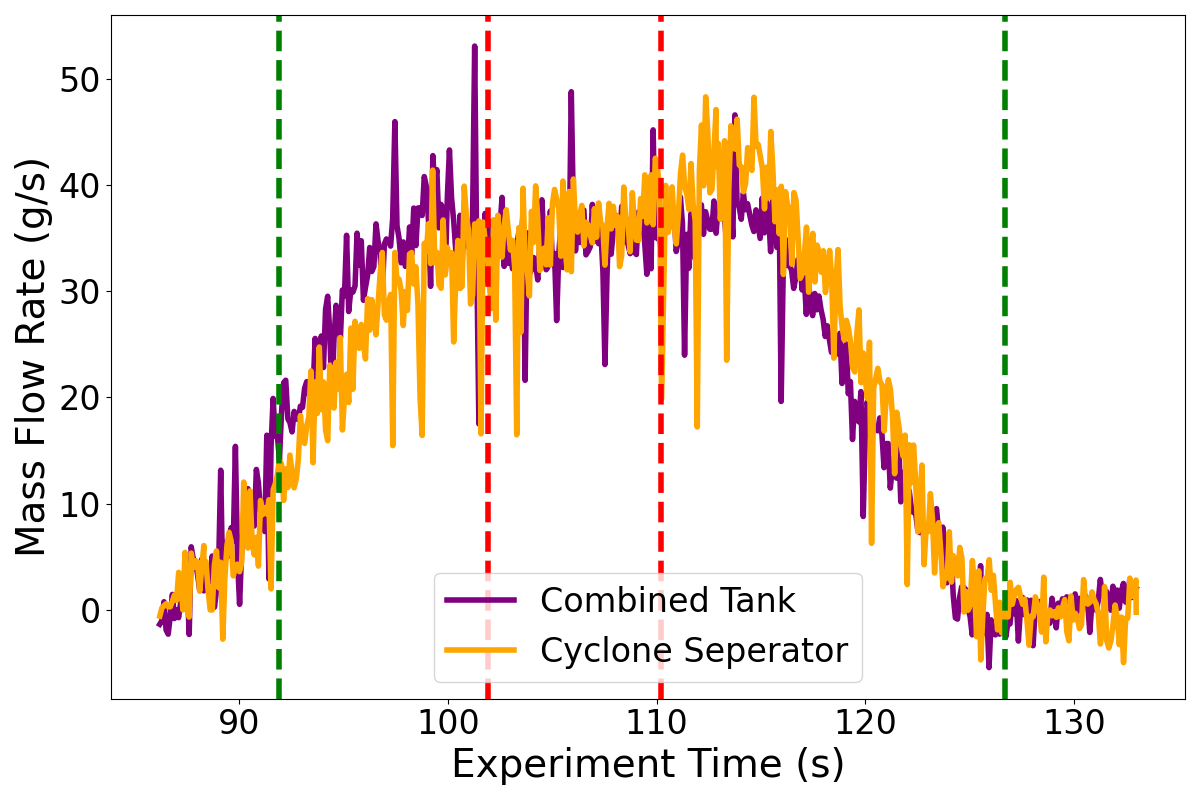
\includegraphics[width=\textwidth]{../report_assets/51_clean_flow_100.png}
        \caption*{(c) Mass Flow Rate}
    \end{minipage}
    \caption{1st Test 5 Bar Inlet}
    
\end{figure}\label{fig:51}
\vfill

\begin{figure}[htbp]
    \centering

    \begin{minipage}{0.32\textwidth}
        \centering
        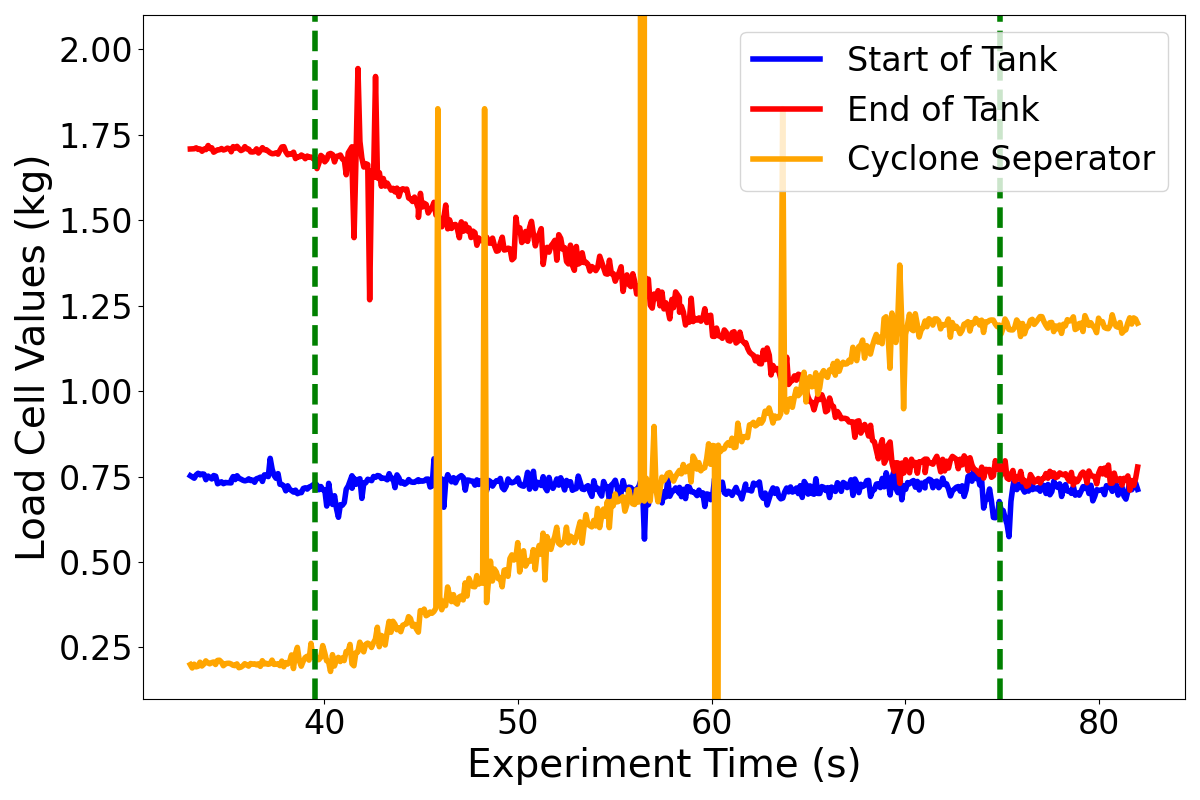
\includegraphics[width=\textwidth]{../report_assets/52_raw_mass.png}
        \caption*{(a) Raw Load Cell Readings}
    \end{minipage}
    \hfill
    \begin{minipage}{0.32\textwidth}
        \centering
        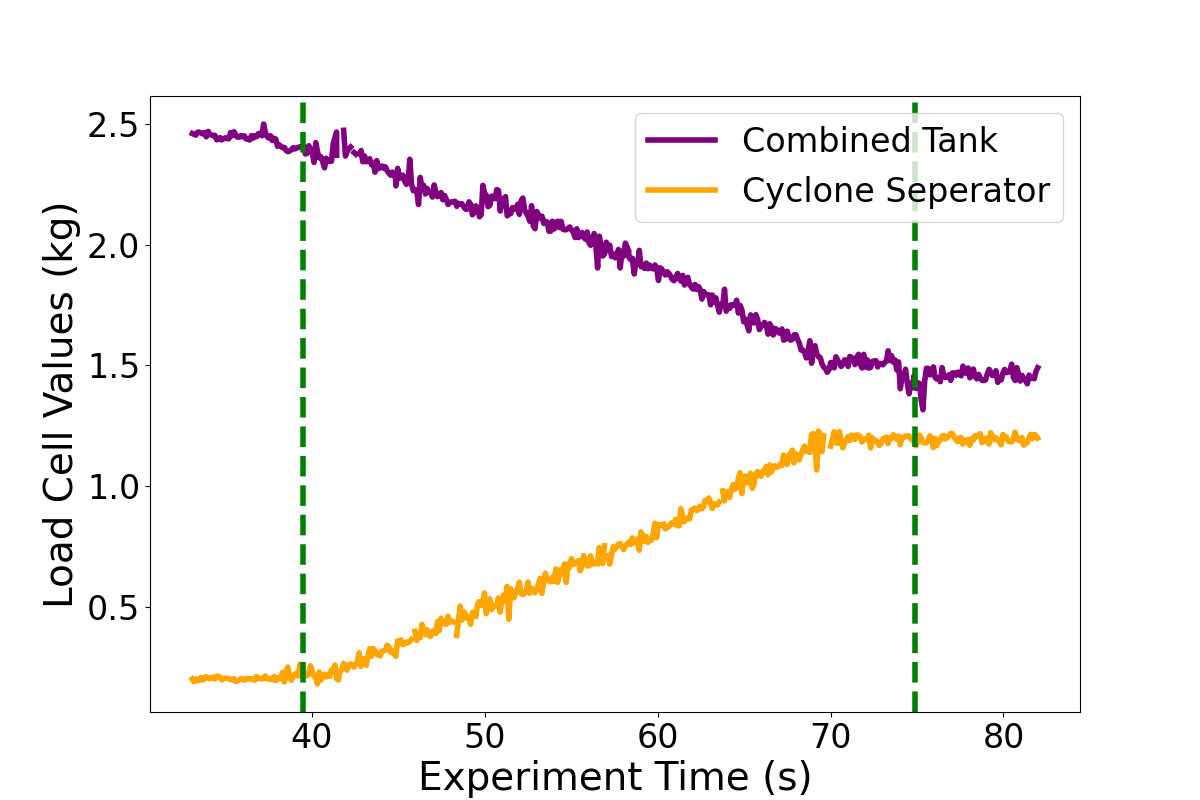
\includegraphics[width=\textwidth]{../report_assets/52_clean_mass.png}
        \caption*{(b) Cleaned Mass Change}
    \end{minipage}
    \hfill
    \begin{minipage}{0.32\textwidth}
        \centering
        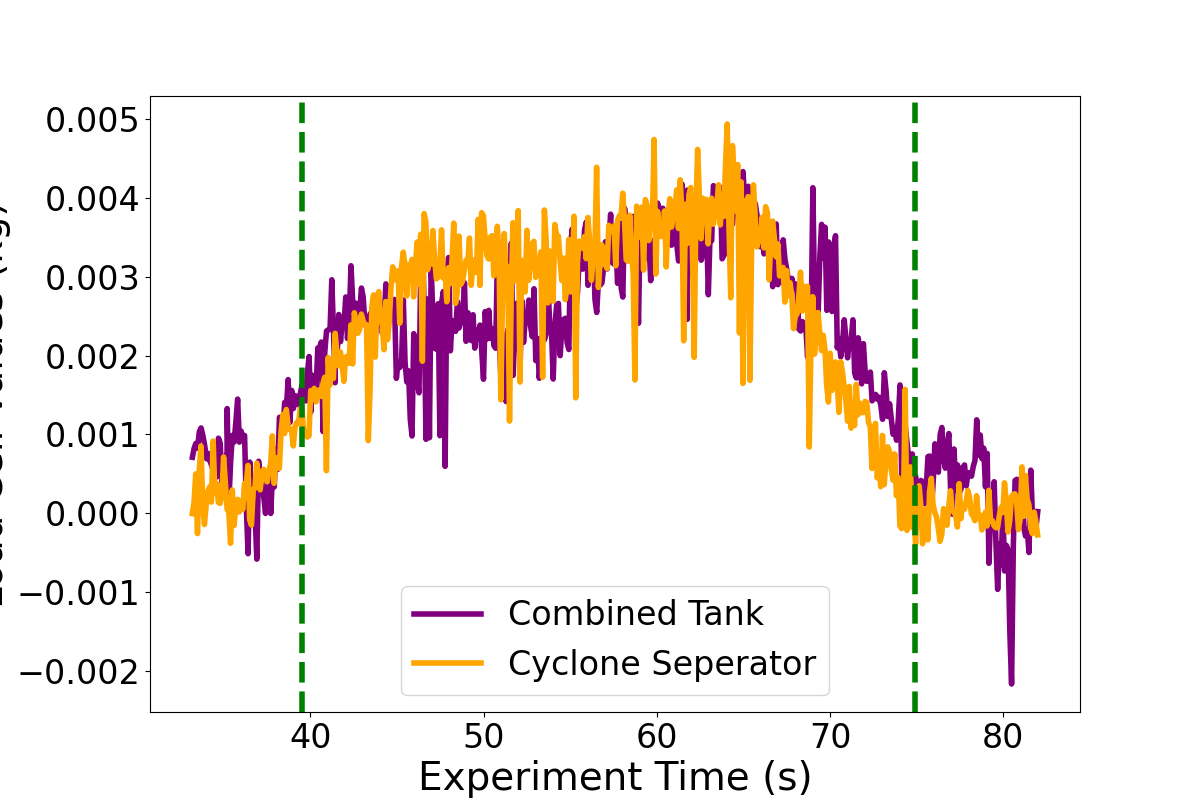
\includegraphics[width=\textwidth]{../report_assets/52_clean_flow_100.png}
        \caption*{(c) Mass Flow Rate}
    \end{minipage}
    \caption{2nd Test 5 Bar Inlet}
    
\end{figure}\label{fig:52}
\vfill

\begin{figure}[htbp]
    \centering

    \begin{minipage}{0.32\textwidth}
        \centering
        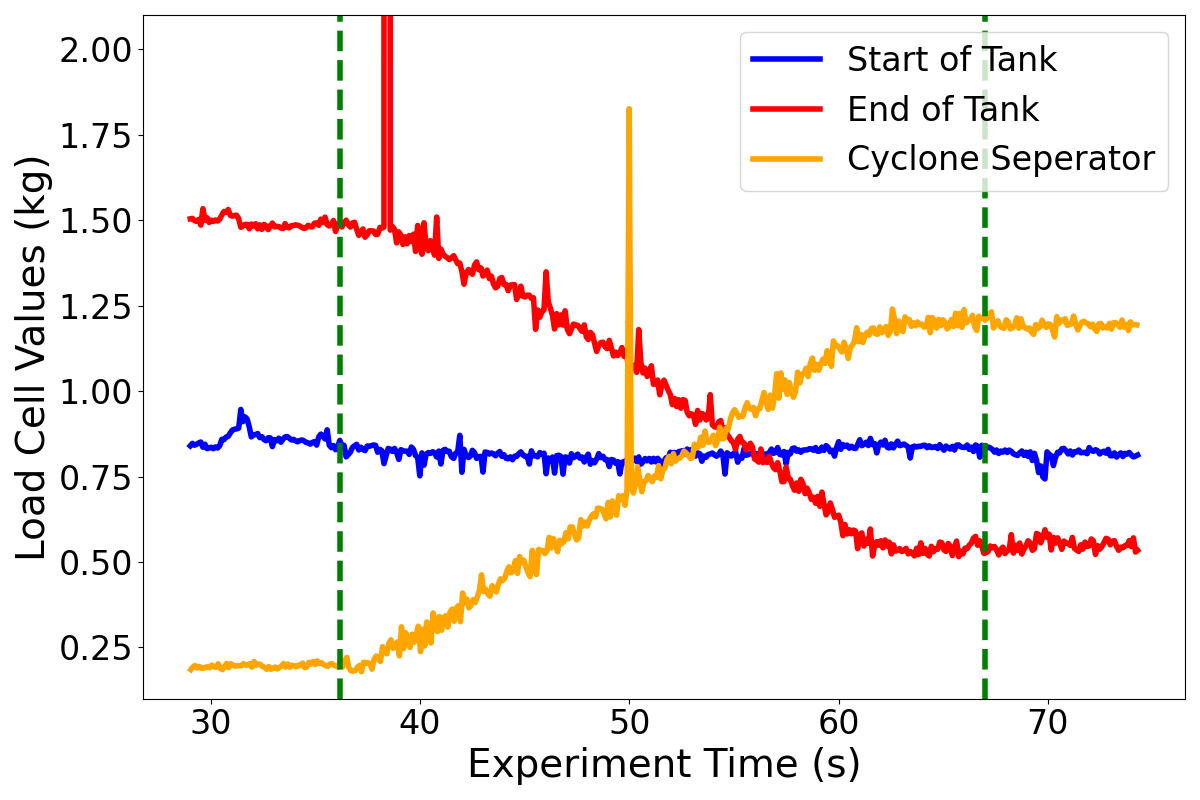
\includegraphics[width=\textwidth]{../report_assets/53_raw_mass.png}
        \caption*{(a) Raw Load Cell Readings}
    \end{minipage}
    \hfill
    \begin{minipage}{0.32\textwidth}
        \centering
        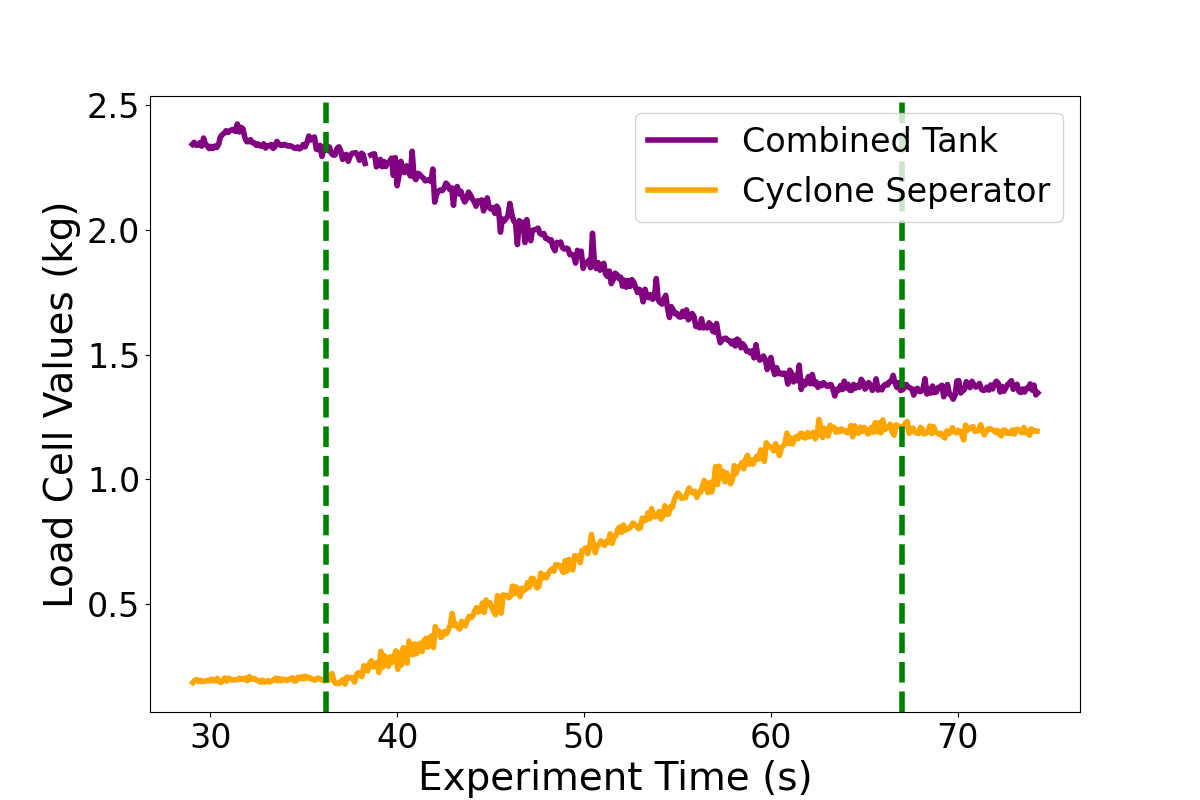
\includegraphics[width=\textwidth]{../report_assets/53_clean_mass.png}
        \caption*{(b) Cleaned Mass Change}
    \end{minipage}
    \hfill
    \begin{minipage}{0.32\textwidth}
        \centering
        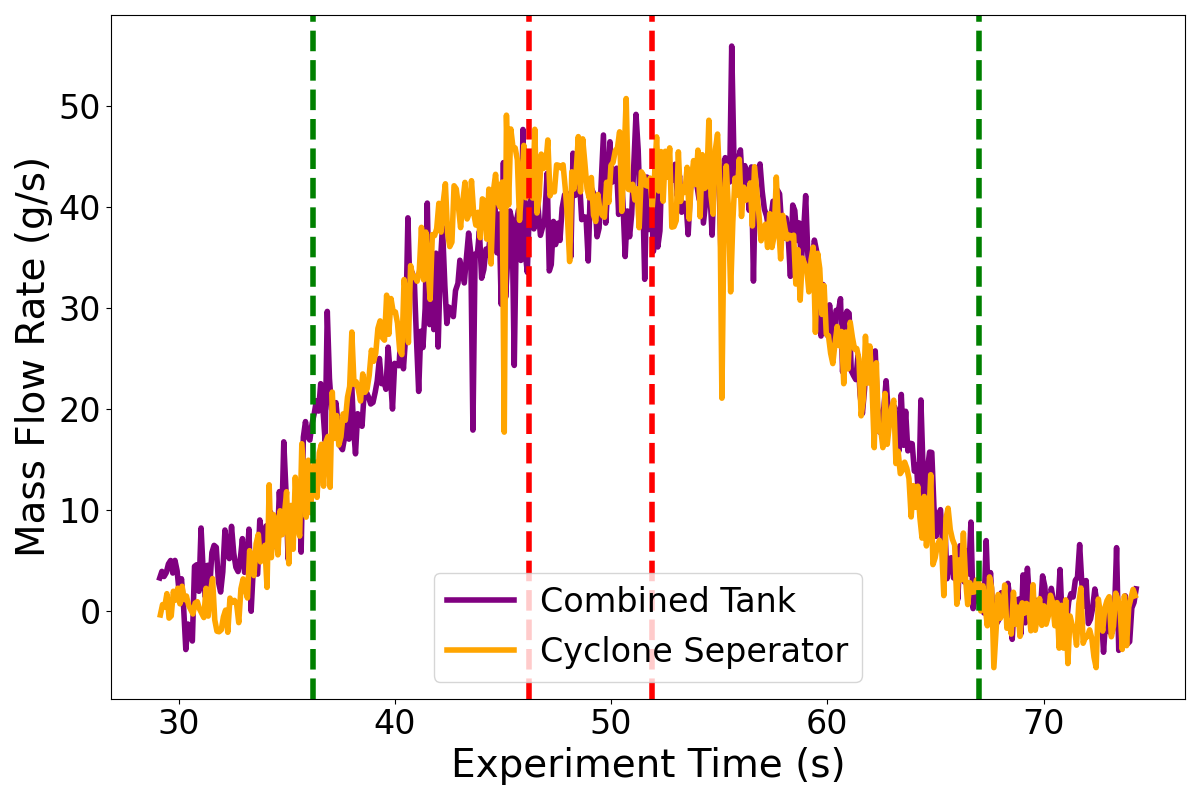
\includegraphics[width=\textwidth]{../report_assets/53_clean_flow_100.png}
        \caption*{(c) Mass Flow Rate}
    \end{minipage}
    \caption{3rd Test 5 Bar Inlet}
    
\end{figure}\label{fig:53}
\vfill
\newpage

\subsection{Results from an Inlet Pressure of 6 bar}
\vfill
\begin{figure}[htbp]
    \centering

    \begin{minipage}{0.32\textwidth}
        \centering
        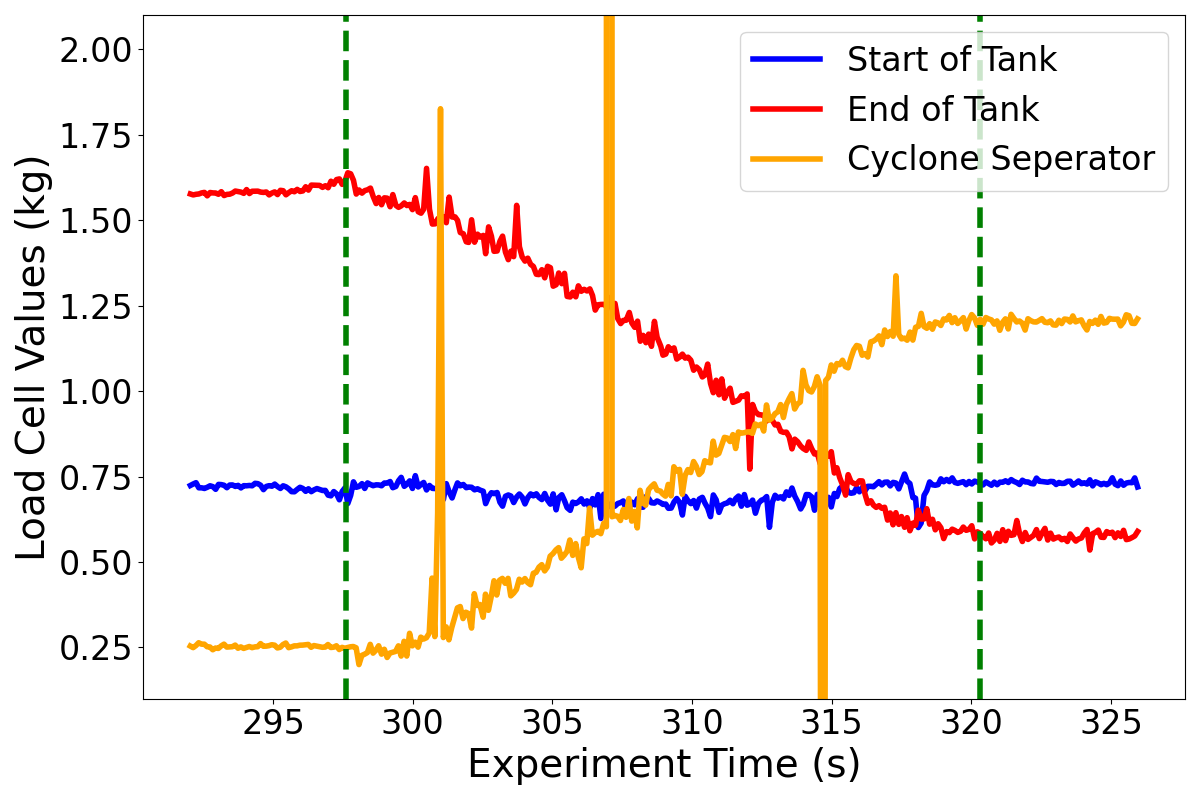
\includegraphics[width=\textwidth]{../report_assets/61_raw_mass.png}
        \caption*{(a) Raw Load Cell Readings}
    \end{minipage}
    \hfill
    \begin{minipage}{0.32\textwidth}
        \centering
        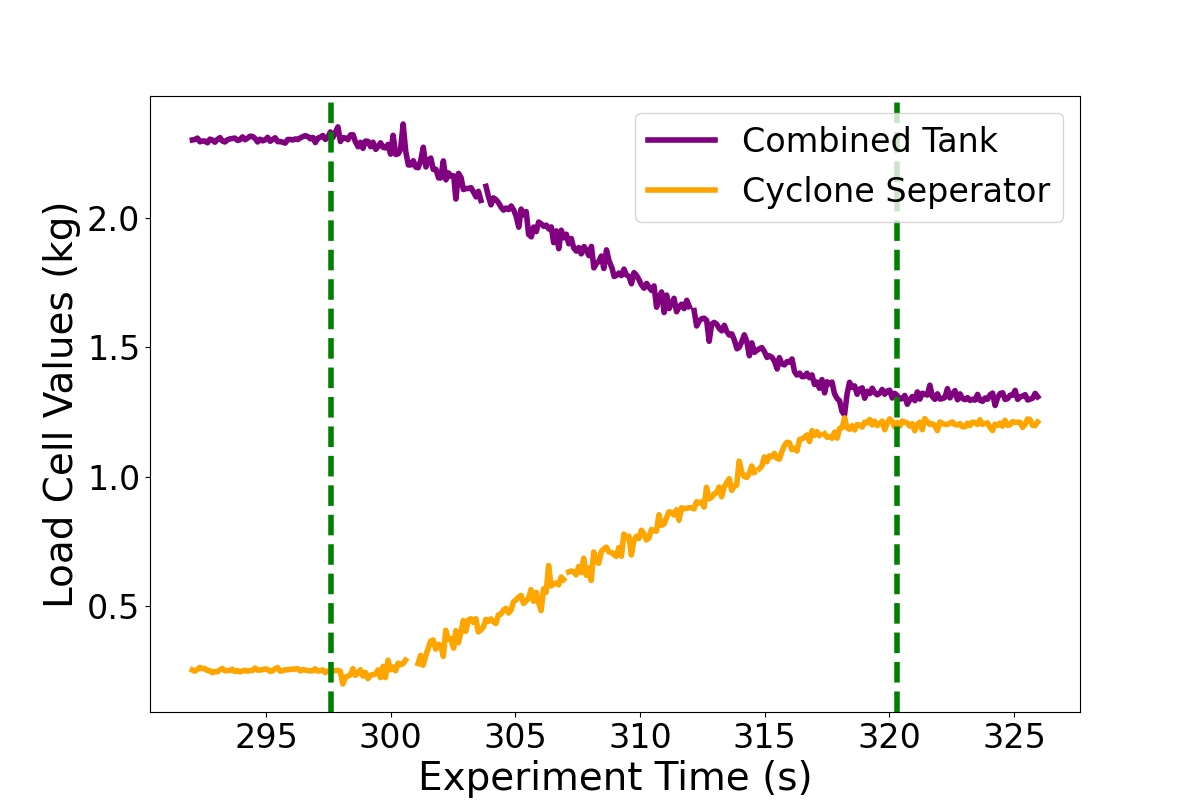
\includegraphics[width=\textwidth]{../report_assets/61_clean_mass.png}
        \caption*{(b) Cleaned Mass Change}
    \end{minipage}
    \hfill
    \begin{minipage}{0.32\textwidth}
        \centering
        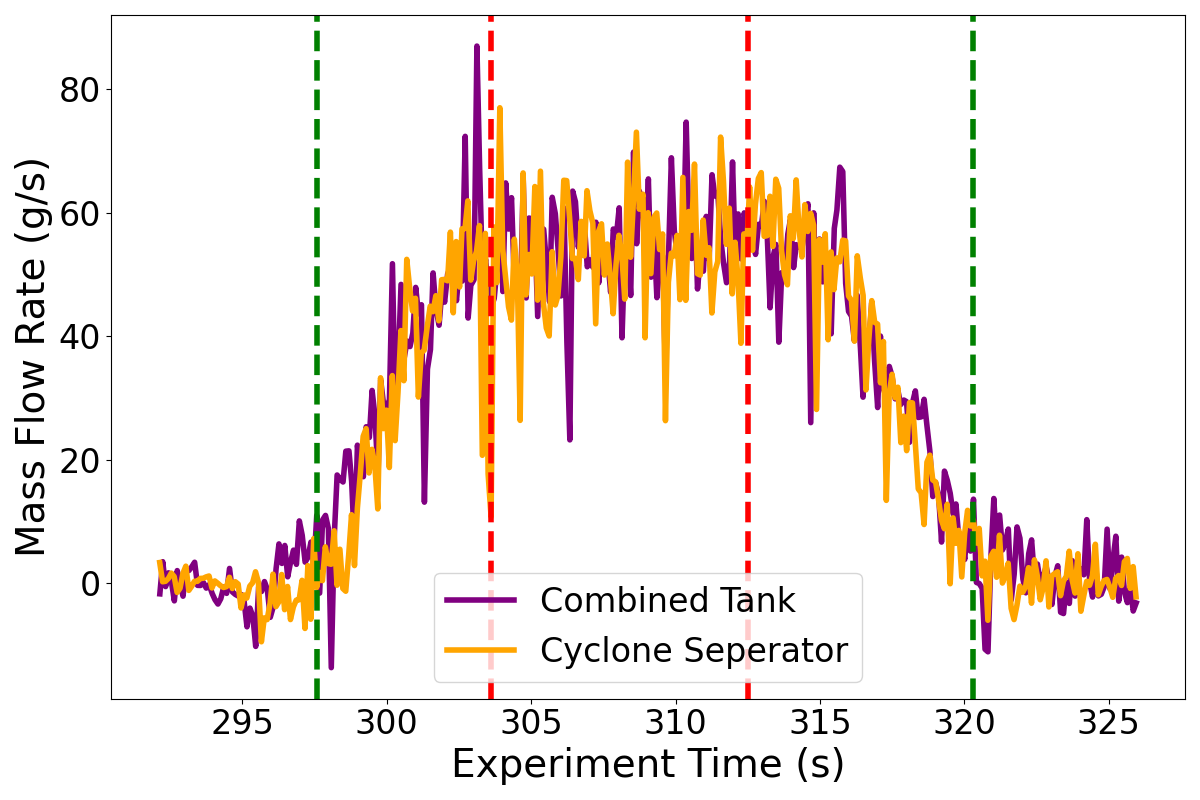
\includegraphics[width=\textwidth]{../report_assets/61_clean_flow_50.png}
        \caption*{(c) Mass Flow Rate}
    \end{minipage}
    \caption{1st Test 6 Bar Inlet}
    
\end{figure}\label{fig:61}

\vfill
\begin{figure}[htbp]
    \centering

    \begin{minipage}{0.32\textwidth}
        \centering
        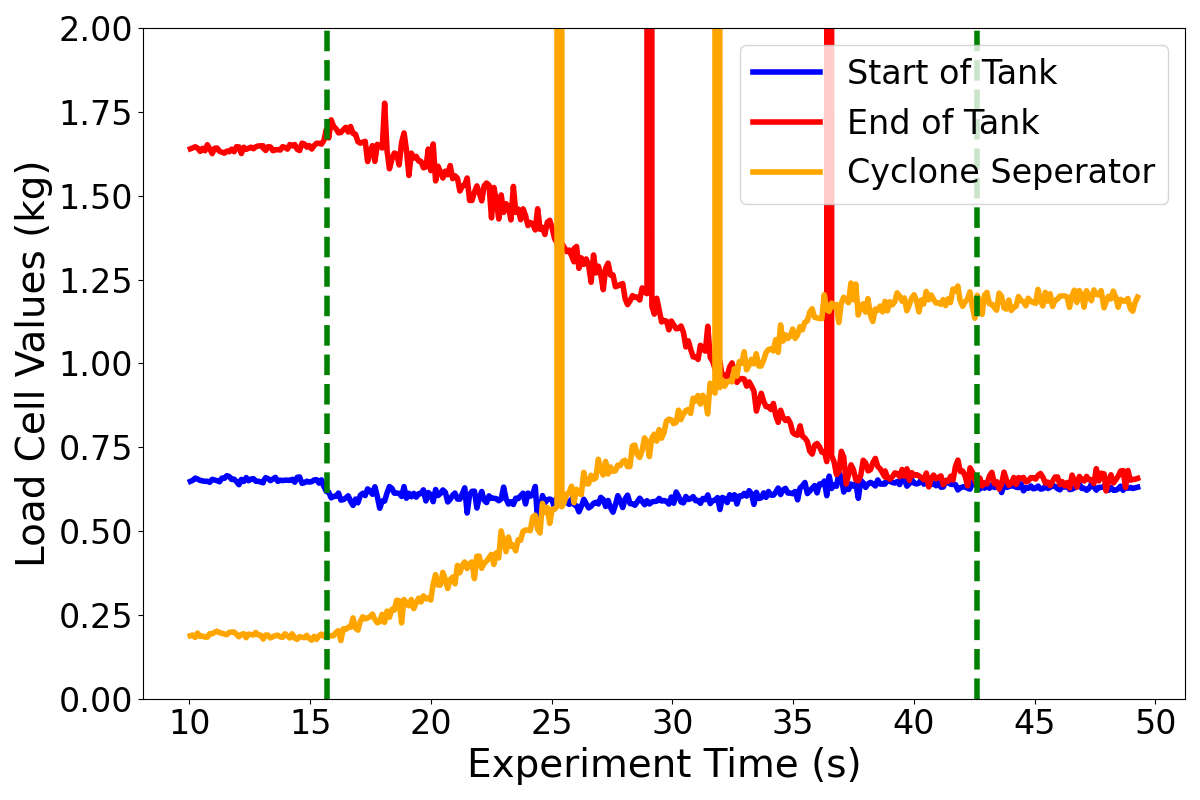
\includegraphics[width=\textwidth]{../report_assets/63_raw_mass.png}
        \caption*{(a) Raw Load Cell Readings}
    \end{minipage}
    \hfill
    \begin{minipage}{0.32\textwidth}
        \centering
        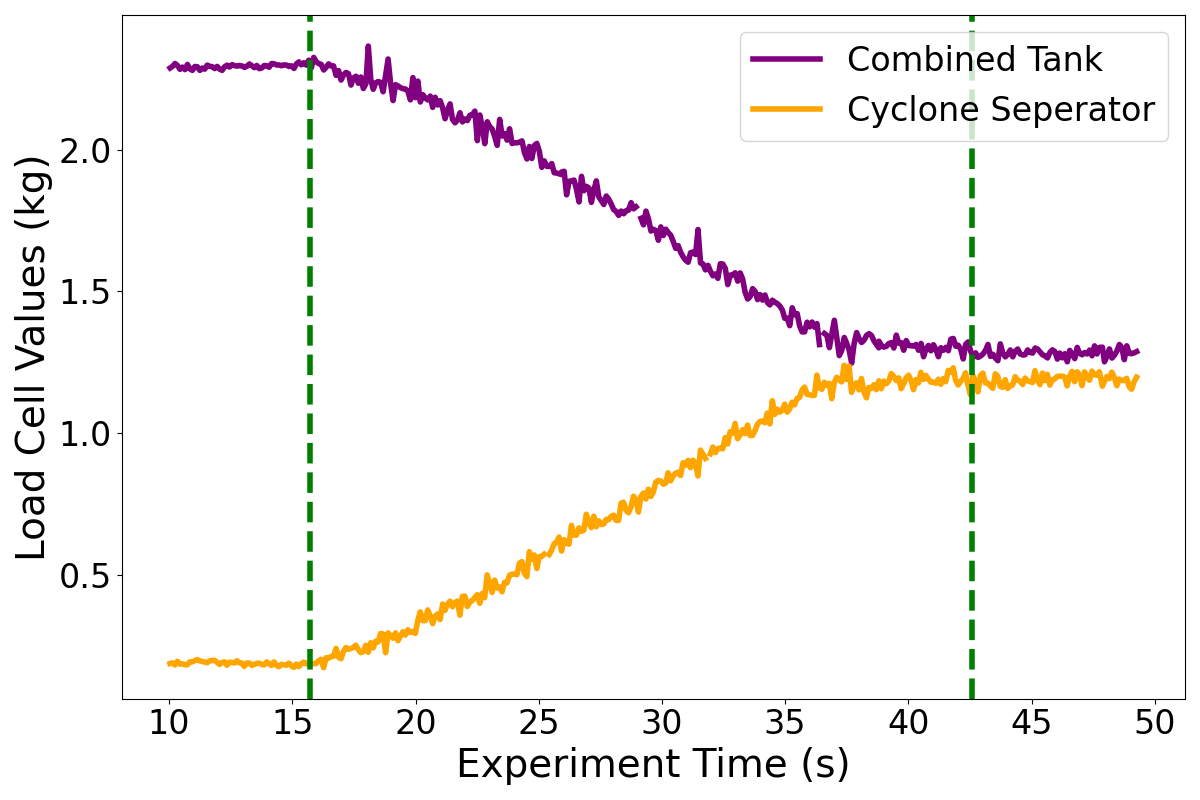
\includegraphics[width=\textwidth]{../report_assets/63_clean_mass.png}
        \caption*{(b) Cleaned Mass Change}
    \end{minipage}
    \hfill
    \begin{minipage}{0.32\textwidth}
        \centering
        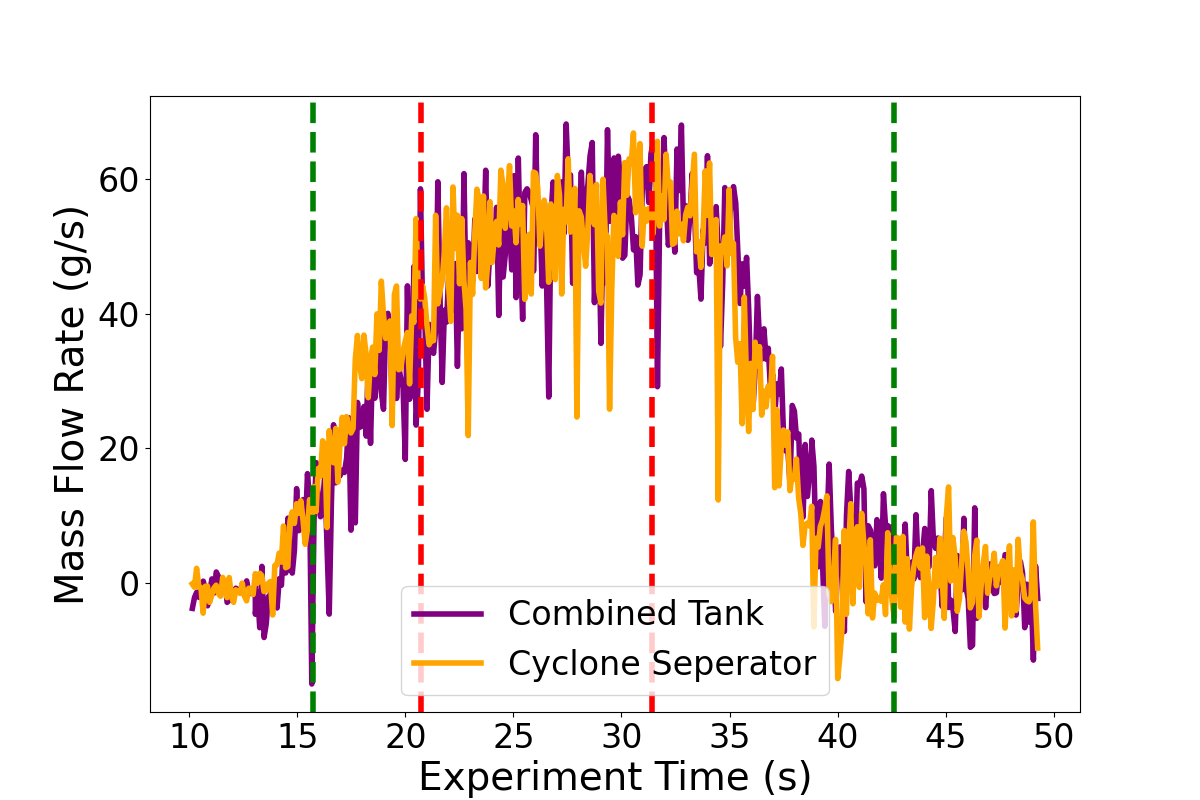
\includegraphics[width=\textwidth]{../report_assets/63_clean_flow_50.png}
        \caption*{(c) Mass Flow Rate}
    \end{minipage}
    \caption{2nd Test 6 Bar Inlet}
    
\end{figure}\label{fig:63}

\vfill
\begin{figure}[htbp]
    \centering

    \begin{minipage}{0.32\textwidth}
        \centering
        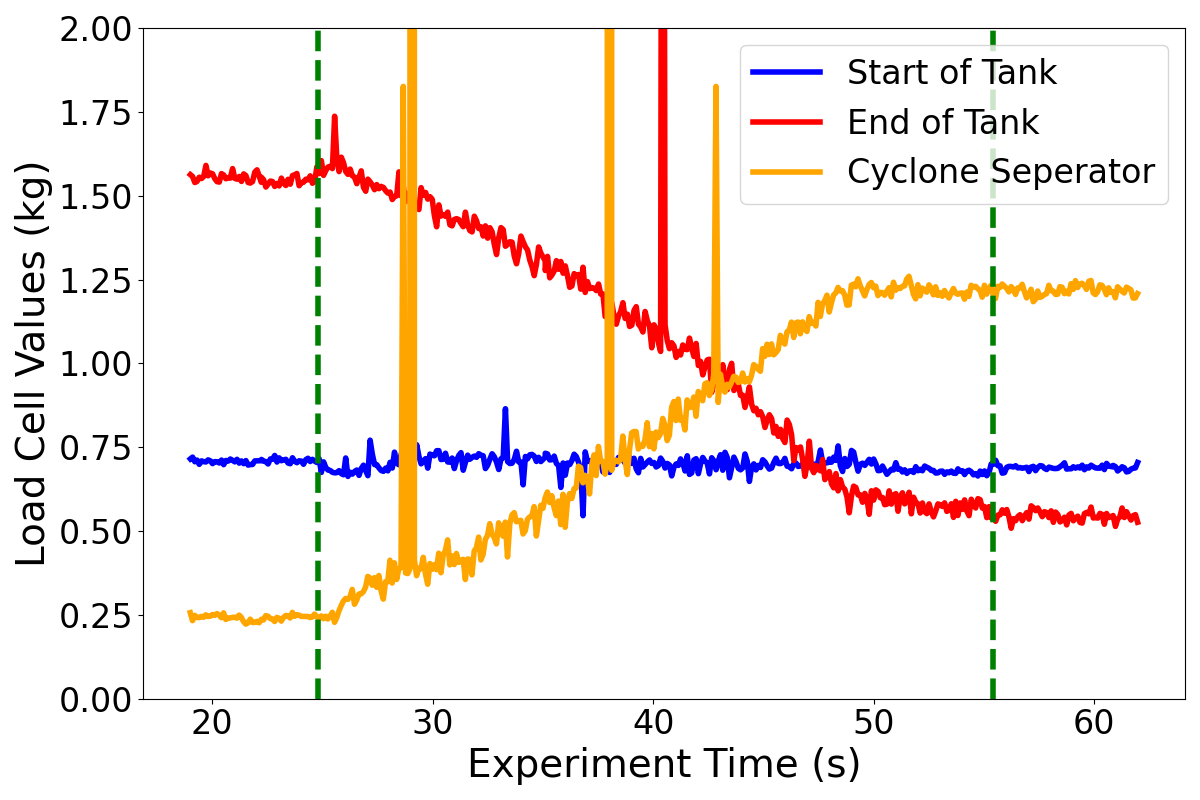
\includegraphics[width=\textwidth]{../report_assets/64_raw_mass.png}
        \caption*{(a) Raw Load Cell Readings}
    \end{minipage}
    \hfill
    \begin{minipage}{0.32\textwidth}
        \centering
        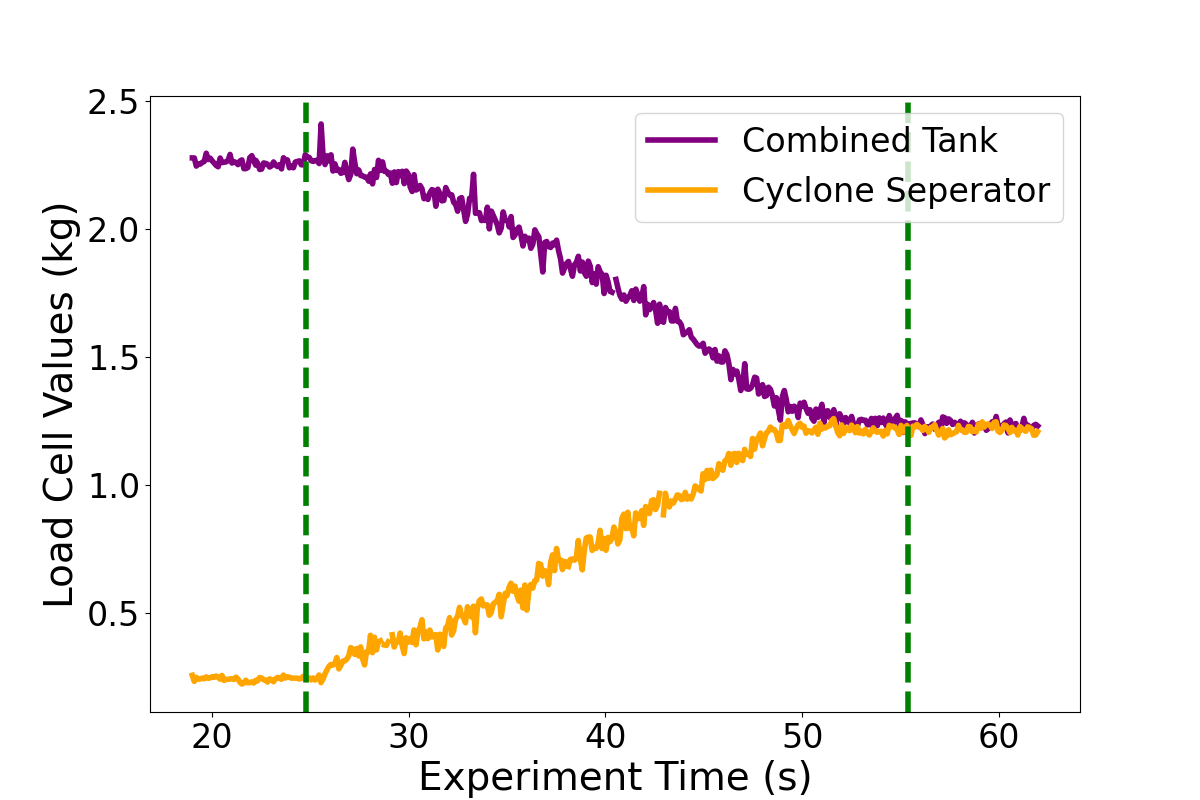
\includegraphics[width=\textwidth]{../report_assets/64_clean_mass.png}
        \caption*{(b) Cleaned Mass Change}
    \end{minipage}
    \hfill
    \begin{minipage}{0.32\textwidth}
        \centering
        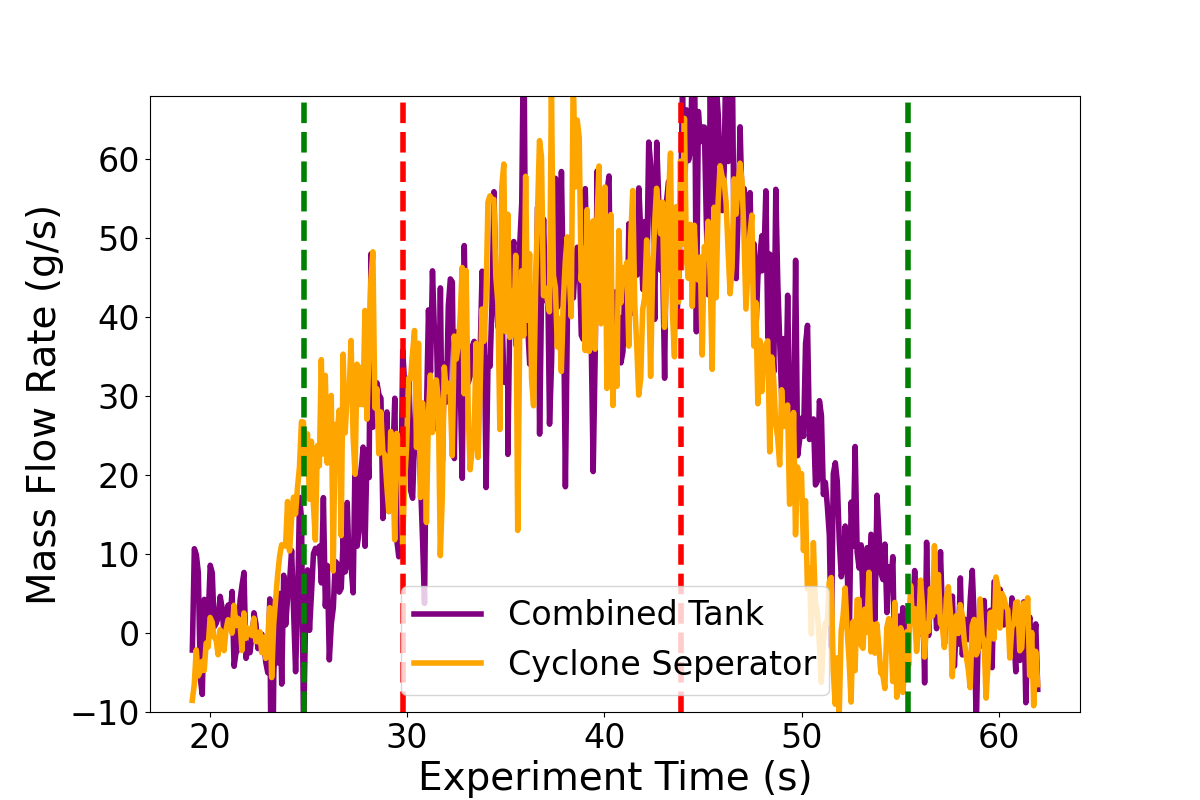
\includegraphics[width=\textwidth]{../report_assets/64_clean_flow_50.png}
        \caption*{(c) Mass Flow Rate}
    \end{minipage}
    \caption{3rd Test 6 Bar Inlet}
    
\end{figure}\label{fig:64}
\vfill
\newpage

\subsection{Mass Flow Rate Analysis and Discussion}
For each of the tests, the raw load cell readings can be seen on graph a. Most graphs show that there was noise in the readings resulting in a few data points being drastically larger or smaller than the surrounding data. While steps were taken to prevent this, like taping down the screw terminal incase the problem was a faulty wire connections, they never fixed the issue. The fact that the noise is less common in the lower pressure recordings implies that this could be somehow caused by electrostatic charge buildup in the sand from the triboelectric effect. These anomolous results were removed by hand and the load cell data from the start and the end of the tank were added together to find the mass leaving the whole tank over time seen in graph b. Finally, from the two mass measurements a simple moving average was calculated with a window of 100 data points for the 4 and 5 bar inlet pressure tests and a window of 50 data points for the 6 bar inlet pressure tests. The polling rate of the sensors was 10Hz so with a 100 data point moving window, data up to 10s after the opening of the valve will be affected by edge distortion. The green dashed lines on the graphs indicate the time where the valves were opened or closed, while the red dashed lines represent data that should be unaffected by edge distortion. This was prescribed as being 10 seconds after the opening of the valve and 10s before the mass change plateaued for the 4 and 5 bar inlet pressure test; the 6 bar test used 5s correspondingly.

The first thing to note from the tests is the large variation between the shapes of the mass flow rate even within tests of the same inlet pressure. Comparing the mass flow rate for all tests with a 4 bar pressure inlet shows this phenomenon.  Even reducing the analysis to the data within the red dashed lines still highlights the variability. Even more problematic is the gradient of mass flow rate. Test 1 starts at around 18g/s and then finishes at 25g/s, test 2 starts at 21g/s and ends at 28g/s and test 3 starts and ends around 29g/s. A slight increase over time of mass flow rate would be expected as there is less powder in the tank to lower the static pressure the fluidising region sees. The difference in change in mass flow rate over time between the first two tests and the final one does cast doubt on the systems ability to dispense powder at a consistent mass flow rate. Both the gradient of the mass flow rate and the magnitude are varying between tests.

Other interesting behaviours are \autoref{fig:52} (c), which shows a relatively large divergence of mass flow rates calculated between the two methods. Upon reviewing the video recording of this test it is not apparent what caused this result as it was conducted the same as the tests before and after it and visually, behaved the same.

The final significant result of the testing is the mass flow rate range of 20g/s to 60g/s. This is 3 orders of magnitude higher than previous systems, reporting feed rates of 3.5 and 5.7 grams a minute~\cite{BHATTIPROLU20181}. While this strongly supports the scalability of fluidising powder feed systems, it weakens the parallels that can be drawn between the behaviour of this system and others in literature. To address this, the chokepoint could be reintroduced given the powder size is reduced to prevent the clogging issue. This could, however, reduce the pressure differential seen by the piston leading to a reduced packing efficacy.

\subsection{System Behaviour}
The system behaviour differed greatly to expectations outlined in \autoref{sec:expected-behaviour}. 